\def\fileversion{v2.25b} \def\filedate{2014/05/02}
% \iffalse  % this is a METACOMMENT !
%% Package and Class "uiucthesis2014" for use with LaTeX2e.
%
%<class|package>\NeedsTeXFormat{LaTeX2e}
%<class>\ProvidesClass{uiucthesis2014}
%<package>\ProvidesPackage{uiucthesis2014}
%<class|package>         [\filedate\ \fileversion\ UIUC Thesis (PJC)]
%
%<*driver>
\documentclass{ltxdoc}
\begin{document}
\title{The \textsf{uiucthesis2014} class
       \thanks{This file has version number \fileversion,
       last revised \filedate.}}
\author{Charles Kiyanda\\charles@kiyanda.com\\(Adapted from version 2.25, 2005/03/25 by Peter Czoschke\\Updated in 2007 by Tim Head.)}
\date{\filedate}
\maketitle
\DocInput{uiucthesis2014.dtx}
\end{document}
%</driver>
% \fi
%
% \CheckSum{1158}
%
% \MakeShortVerb{\|}
%
% \def\pkg#1{\textsf{#1}}
% \def\env#1{\textsf{#1}}
%
% \iffalse
%<*example>
% \fi
% \begin{abstract}
% Load the \pkg{uiucthesis2014} class for use with \LaTeX2e
% to produce a document that should conform
% to the format described in
% \emph{Handbook for Graduate Students Preparing to Deposit}\cite{Handbook}. (Actually
% I have checked the requirements from a grad college webpage\cite{thesisweb}.
% I believe 
% this template complies, but there is no guarantee.)
% \end{abstract}
% 
% \section{The User Interface}
%
% This section describes how to use the \pkg{uiucthesis2014} class to
% produce a thesis satisfying the format requirements of the
% Grad College at UIUC.
% I assume that you are familiar with \LaTeX, and highly
% recommend that anyone attempting to use \LaTeX\ to produce a
% thesis have access to a copy of the \LaTeX\ book\cite{Lamport}.
%
% Note that I haven't graduated yet and so I haven't taken this template
% through the ultimate test, which is to actually submit a thesis that ues it.
% I believe this template does conform to the graduate college requirement, but I am,
% \emph{in no way} guaranteeing it conforms to anything.
%
% Also, I'm writing my thesis right now as well. I don't plan to make any more changes to this
% template until I graduate. Hence, if you send me an e-mail right now asking to change some
% detail that you'd think looks better, you're likely to either
% not get a response or receive a somewhat polite ``Wait until january...'' type of response.
% If you firmly believe this template does not conform to the graduate college requirements, be
% very precise and I might look at it. It's just the way it is right now, I'm afraid...
% 
% \subsection{Using \pkg{uiucthesis2014}}
%
% To write a thesis, you load the UIUC thesis definitions
% by loading the \pkg{uiucthesis2014} class at the beginning of
% your \LaTeX\ document with the |\documentclass| command.
% For example,
% \begin{quote} \hrule \begin{verbatim}
\documentclass[edeposit,fullpage]{uiucthesis2014}
% \end{verbatim} \hrule \end{quote}
% \iffalse
%<example>
% \fi
%
% \DescribeMacro{[draftthesis]}
% \DescribeMacro{[fancy]}
% \DescribeMacro{[fullpage]}
% The \pkg{uiucthesis2014} class provides a number of options.
% The |[draftthesis]| option causes each page to have a header
% proclaiming the document to be a draft copy, along with the
% current time and date.
% It also omits the copyright page and prints out any marginal notes
% added with the |\note| macro.
% The |[fancy]| style option produces slightly fancier chapter headings.
% The |[fullpage]| style option makes the margins as small as the
% format requirements allow and uses double-spacing for the text.
% Because wide text columns are generally
% considered harder on the reader
% this is not the default, but is provided as an option because people
% seem to want it.
% The |[fancy]| and |[fullpage]| options are incompatible---choose
% one or the other.
%
% \DescribeMacro{[proquest]}
% The |[proquest]| option is meant to be used when you are ready to deposit your thesis.
% For doctorates, the Grad College requires the submission of a specially
% formatted abstract for the ProQuest publication service. To produce this
% abstract, include the |[proquest]| option and reprocess your file. Everything
% in your \LaTeX\ document will be ignored except the contents of the \env{abstract}
% environment, which are printed out in the format required. Once the option is
% removed from the |\documentclass| command, you can reprocess your thesis as
% normal (the auxiliary files should be intact). To use this option, the name
% of your thesis advisor needs to be specified with the |\advisor| command (see
% below).
%
% \DescribeMacro{[edeposit]}
% Use the |[edeposit]| option if you are depositing your thesis electronically. The title page
% used to be different, but the requirement appears to have been harmonized since. The page 
% numbering is slightly different since the committee
% approval form is not included with your thesis. (The page numbering change is currently the
% only difference of thet edeposit option.  You
% must specify your committee members with the |\committee| command (see below).
%
% \DescribeMacro{[offcenter]}
% The |[offcenter]| option adds 1/2 inch to the left margin of all pages and takes
% away 1/2 inch to the text width, leaving a 1.5in left margin and a 1in right margin.
% I believe this setting satisfies the pre-2009 requirement by the grad college to
% have a 1.5in margin for binding. It should also allow you more room for binding
% if you need it. The new requirement is a minimum 1in margin all around and the 
% |[fullpage]| option without the |[offcenter]| option should achieve this goal.
%
% This can now be done to allow some extra space there for binding purposes, or
% if you use the |[fancy]| option, to allow for more space for the chapter
% numbers at the left side of the page.
% In past versions of \pkg{uiucthesis2014} (the name used was simply uiucthesis)
% , the |[fancy]| option did this by default.
% This version uses symmetric margins by default, even with the
% |[fancy]| option. If you have a lot of chapters (i.e., more than 9), your chapter
% numbers may spill into
% the 1 inch margin required by the Grad College without using this option.
%
% \DescribeMacro{[centerchapter]}
% Normally, the chapter headings are all left-justified on the opening page of
% each chapter. These headings can all be centered by using the |[centerchapter]|
% option for the class. This option is not recommended for use with the |[fancy]|
% option.
%
% \subsection{The Title Page}
%
% The |\maketitle| command is redefined so that it creates a
% title page with the correct format for a thesis at UIUC.
%
% \DescribeMacro{\phdthesis}
% \DescribeMacro{\otherdoctorate}
% \DescribeMacro{\msthesis}
% \DescribeMacro{\othermasters}
% \DescribeMacro{\department}
% \DescribeMacro{\college}
% Use the |\phdthesis| or |\msthesis| to set the correct thesis type.
% If your thesis isn't for a ``Ph.D.'' or ``M.S.'', you can specify
% your degree with either\\
% |\otherdoctorate{|\meta{degree name}|}{|\meta{abbreviation}|}| or\\
% |\othermasters{|\meta{degree name}|}{|\meta{abbreviation}|}|.\\
% For example, specifying |\phdthesis| is equivalent to giving the command\\
% |\otherdoctorate{Doctor of Philosophy}{Ph.D.}|.\\
% The default thesis type is |\phdthesis|. Set your department with\linebreak
% |\department{|\meta{department}|}|. This defines the field your degree
% will be in, so leave out ``Department of.''
% The default department is ``Computer Science''.
% Define your college with |\college{|\meta{college}|}|.
% The default is college is ``Graduate College'';
% you shouldn't need to change it.
%
% \DescribeMacro{\schools}
% Use |\schools{|\meta{school list}|}| to list the previous degrees
% you have received and the schools that you received them from.
% Separate multiple degrees with |\\|.
%
% \DescribeMacro{\degreeyear}
% Use |\degreeyear{|\meta{year}|}| to define the year in which
% you will receive your degree.  The default is the current year.
%
% \DescribeMacro{\advisor}
% \DescribeMacro{\adviser}
% Use |\advisor{|\meta{advisor name}|}| or |\adviser{|\meta{advisor name}|}|
% to specify the name of your
% advisor. This is needed to produce the ProQuest abstract
% (see the |[proquest]| option above). You only need to submit a
% ProQuest abstract if you are a doctoral candidate.
%
% \DescribeMacro{\committee}
% Use |\committee{|\meta{committee members}|}| to specify the members
% of your committee and their titles as you want them to appear on the
% title page. Separate members with |\\|. This is needed for
% all forms of thesis submission. To respect the graduate college guidelines,
% you must use the full title of each committee members. The committee chair should
% appear first with the designation ``,chair''. Your thesis adviser should appear second
% with the title ``,Director of Research''. See the graduate college website for details.
%
% \DescribeMacro{\volume}
% The |\volume| macro provides nominal support for very long theses that must
% be broken up into multiple volumes. Use |\volume{|\meta{number}|}|
% to specify the volume number (a single arabic numeral). All this macro
% does is place the word VOLUME with the number you specify on the title
% page. You have to take care of what appears in each volume. The easiest
% way to do this is to create two separate source files, one for each
% volume.
%
% Here's how to produce an example similar to that in \cite{Handbook}.
% \begin{quote} \hrule \begin{verbatim}
\begin{document}

\title{Coffee Consumption of Graduate Students \\
       Trying to Finish Dissertations}
\author{Juan Valdez}
\department{Food Science}
\schools{B.A., University of Columbia, 1981\\
         A.M., University of Illinois at Urbana-Champaign, 1986}
\phdthesis
\advisor{Java Jack}
\degreeyear{1994}
\committee{Professor Prof Uno, Chair\\Professor Prof Dos, Director of Research\\Assistant Professor Prof Tres\\Adjunct Professor Prof Quatro}
\maketitle
% \end{verbatim} \hrule \end{quote}
% \iffalse
%<example>
% \fi
%
% \subsection{Front Matter}
%
% \DescribeMacro{\frontmatter}
% Typically, a thesis might have an Abstract, a Dedication, some
% Acknowledgments, and a Preface before the Table of Contents.
% Use the |\frontmatter| command to start this preliminary section
% of the thesis.
% The |\frontmatter| command sets the page number of the next page
% to roman numeral iii (or ii if the |[edeposit]| option is used).
% (The title page is page i, and the certificate
% of committee approval, the ``red-bordered form,'' is page ii.)
%
% \DescribeEnv{abstract}
% The abstract should appear in the \env{abstract} environment. Normally,
% this just produces another chapter with |\chapter*{\abstractname}|,
% where |\abstractname| is ``Abstract'' (see User Customization below),
% but if the |[proquest]| option
% is specified, then the contents of this environment are used
% for the ProQuest abstract.
%
% \DescribeEnv{dedication}
% A dedication page can be printed with the \env{dedication} environment.
% This produces a separate page with the dedication centered horizontally
% and vertically, with the text in italics.
%
% After this front matter comes the Table of Contents,
% List of Tables, List of Figures, etc.  Use the standard \LaTeX\
% commands |\tableofcontents|, |\listoftables|, |\listoffigures|, etc.,
% to generate them.
% In the \pkg{uiucthesis2014} format these lists are all single spaced.
%
% \DescribeEnv{symbollist}
% \DescribeEnv{symbollist*}
% Optionally, these tables can be followed by a List of Abbreviations and/or
% List of Symbols. Introduce these with the |\chapter| command. To aid in
% making these lists, the \env{symbollist} and \env{symbollist*} environments are
% defined in \pkg{uiucthesis2014}. These environments produce a two-column list
% as illustrated below. By default the left column is 1 inch wide but can
% be specified with an optional argument. In the starred environment, the left
% column is left-justified, otherwise it is centered. See the example below.
%
% Here's an example of what the front matter of a typical
% thesis looks like.  First comes the Abstract and the Dedication, both of
% which are optional.
% \begin{quote} \hrule \begin{verbatim}
\frontmatter

%% Create an abstract that can also be used for the ProQuest abstract.
%% Note that ProQuest truncates their abstracts at 350 words.
\begin{abstract}
This is a comprehensive study of caffeine consumption by graduate
students at the University of Illinois who are in the very final
stages of completing their doctoral degrees. A study group of six
hundred doctoral students\ldots.
\end{abstract}

%% Create a dedication in italics with no heading, centered vertically
%% on the page.
\begin{dedication}
To Father and Mother.
\end{dedication}

%% Create an Acknowledgements page, many departments require you to
%% include funding support in this.
\chapter*{Acknowledgments}

This project would not have been possible without the support of
many people. Many thanks to my adviser, Lawrence T. Strongarm, who
read my numerous revisions and helped make some sense of the
confusion. Also thanks to my committee members, Reginald Bottoms,
Karin Vegas, and Cindy Willy, who offered guidance and support.
Thanks to the University of Illinois Graduate College for awarding
me a Dissertation Completion Fellowship, providing me with the
financial means to complete this project. And finally, thanks to
my husband, parents, and numerous friends who endured this long
process with me, always offering support and love.

%% The thesis format requires the Table of Contents to come
%% before any other major sections, all of these sections after
%% the Table of Contents must be listed therein (i.e., use \chapter,
%% not \chapter*).  Common sections to have between the Table of
%% Contents and the main text are:
%%
%% List of Tables
%% List of Figures
%% List Symbols and/or Abbreviations
%% etc.

\tableofcontents
\listoftables
\listoffigures
% \iffalse
%<example>
% \fi
% \end{verbatim} \hrule \end{quote}
%
% If you want a List of Symbols or Abbreviations, you can do so as follows:
% \begin{quote} \hrule \begin{verbatim}
%% Create a List of Abbreviations. The left column
%% is 1 inch wide and left-justified
\chapter{List of Abbreviations}

\begin{symbollist*}
\item[CA] Caffeine Addict.
\item[CD] Coffee Drinker.
\end{symbollist*}

%% Create a List of Symbols. The left column
%% is 0.7 inch wide and centered
\chapter{List of Symbols}

\begin{symbollist}[0.7in]
\item[$\tau$] Time taken to drink one cup of coffee.
\item[$\mu$g] Micrograms (of caffeine, generally).
\end{symbollist}
% \end{verbatim} \hrule \end{quote}
% \iffalse
%<example>
% \fi
%
% \subsection{Main Matter}
%
% \DescribeMacro{\mainmatter}
% Begin the main body of your thesis with the |\mainmatter| command.
% It resets the page number to arabic numeral 1.
% You can now use any of the commands defined by the
% the book document class to write your thesis.
%
% In the following example, each of the chapters
% has been broken out into separate files that are inserted into
% this main file with the |\include| command.  This allows the
% thesis to be proofed quickly while it is being revised with
% the |\includeonly| command.  To provide an example of what the
% chapter headings look like, one chapter has been explicitly
% coded. (Try recompiling the example file with the |[fancy]|
% option instead of |[fullpage]| to see the effect.)
%
% \begin{quote} \hrule \begin{verbatim}
\mainmatter
% Sample chapter to test margins
\chapter{This world}
\section{Of the Nature of Flatland}


I call our world Flatland, not because we call it so, but to make its
nature clearer to you, my happy readers, who are privileged to live in
Space.

Imagine a vast sheet of paper on which straight Lines, Triangles,
Squares, Pentagons, Hexagons, and other figures, instead of remaining
fixed in their places, move freely about, on or in the surface, but
without the power of rising above or sinking below it, very much like
shadows--only hard with luminous edges--and you will then have a pretty
correct notion of my country and countrymen.  Alas, a few years ago, I
should have said "my universe:"  but now my mind has been opened to
higher views of things.

In such a country, you will perceive at once that it is impossible that
there should be anything of what you call a "solid" kind; but I dare
say you will suppose that we could at least distinguish by sight the
Triangles, Squares, and other figures, moving about as I have described
them.  On the contrary, we could see nothing of the kind, not at least
so as to distinguish one figure from another.  Nothing was visible, nor
could be visible, to us, except Straight Lines; and the necessity of
this I will speedily demonstrate.

Place a penny on the middle of one of your tables in Space; and leaning
over it, look down upon it.  It will appear a circle.

But now, drawing back to the edge of the table, gradually lower your
eye (thus bringing yourself more and more into the condition of the
inhabitants of Flatland), and you will find the penny becoming more and
more oval to your view, and at last when you have placed your eye
exactly on the edge of the table (so that you are, as it were, actually
a Flatlander) the penny will then have ceased to appear oval at all,
and will have become, so far as you can see, a straight line.

The same thing would happen if you were to treat in the same way a
Triangle, or a Square, or any other figure cut out from pasteboard.  As
soon as you look at it with your eye on the edge of the table, you will
find that it ceases to appear to you as a figure, and that it becomes
in appearance a straight line.  Take for example an equilateral
Triangle--who represents with us a Tradesman of the respectable class.
Figure 1 represents the Tradesman as you would see him while you were
bending over him from above; figures 2 and 3 represent the Tradesman,
as you would see him if your eye were close to the level, or all but on
the level of the table; and if your eye were quite on the level of the
table (and that is how we see him in Flatland) you would see nothing
but a straight line.

When I was in Spaceland I heard that your sailors have very similar
experiences while they traverse your seas and discern some distant
island or coast lying on the horizon.  The far-off land may have bays,
forelands, angles in and out to any number and extent; yet at a
distance you see none of these (unless indeed your sun shines bright
upon them revealing the projections and retirements by means of light
and shade), nothing but a grey unbroken line upon the water.

Well, that is just what we see when one of our triangular or other
acquaintances comes towards us in Flatland.  As there is neither sun
with us, nor any light of such a kind as to make shadows, we have none
of the helps to the sight that you have in Spaceland.  If our friend
comes closer to us we see his line becomes larger; if he leaves us it
becomes smaller; but still he looks like a straight line; be he a
Triangle, Square, Pentagon, Hexagon, Circle, what you will--a straight
Line he looks and nothing else.

You may perhaps ask how under these disadvantagous circumstances we are
able to distinguish our friends from one another: but the answer to
this very natural question will be more fitly and easily given when I
come to describe the inhabitants of Flatland.  For the present let me
defer this subject, and say a word or two about the climate and houses
in our country.

How does this relate to coffee? We direct the reader to \cite{Trembly98}, \cite{Childish07}, and \cite{Presso10}.


\chapter{Introduction}


The economic goal of a society is to maximize wealth by allocating resources efficiently. Capital markets (such as the stock market) provide a method to help allocate resources efficiently. The prediction and inference of future financial events are often critical to achieve the economic goal. Firm specific information contribute to how resources (i.e labor, capital, and natural resources) are allocated in capital markets. The prediction of a future state for a firm (such as the firm's profitability, financial condition, or revenue growth) is an important factor to contribute to how resources should be allocated.  There are many methods used to predict or inform about the future state of a firm.  


\section{Machine Learning}

Machine Learning encompasses a vast set of statistical tools for understanding data and making predictions and inference. These tools fall into supervised or unsupervised categories. For data-driven problems typically we have a response variable (or labels)  referred to as \(Y\) and \(p\) independent variables (or features) refereed to as \(X\). If an assumption is made that there is some relationship between \(Y\) and \(X\) the relationship can be expressed as:

\begin{equation}
\label{eq:function}
Y = f(X) + \epsilon
\end{equation}

\noindent In eq. \ref{eq:function} \(f\) is an unknown function that models the relationship between \(X\) and \(Y\) with  \( \epsilon \) noise.  In most cases it is not possible to perfectly model \(f\) with real-world data and \(f\) is estimated (\(\hat{f}\)). In eq.\ref{eq:function} if \(Y\) is a quantitative variable then regression techniques are used estimate \(f\), however if \(Y\) is a qualitative variable then classification techniques are used.   \(\hat{f}\) is sought for inference where one wants to estimate \(f\) to understand how \(\hat{Y}\) (predicted labels) changes as one adjusts features. \(\hat{f}\) is also sought for prediction where the only concern is the accuracy of predictions for \(Y\). Machine learning provides a variety of approaches to estimate \(f\) for prediction and inference (see \cite{ISL:C1}).

Machine learning problems typically fall into either supervised learning, semi-supervised learning, or unsupervised learning. With supervised learning one wants to fit a model on labels using a set of features. Semi-supervised learning consists of an environment with features and some corresponding labels. Typically in this setting one wishes to use the given features and partial labels to determine what the remaining missing labels are. Lastly with unsupervised learning one has features and no associated labels and seeks to find structure between the features. Currently, the research in this book will only utilize supervised learning. 

\subsection{Supervised Learning} \label{sec:SupervisedLearning}
In a supervised learning paradigm it is not enough to only have \(\hat{f}\) estimate \(f\) well on a dataset. \(\hat{f}\) is often sought to learn a dataset well enough to generalize well to new data that  \(\hat{f}\) has never seen before. To achieve this goal, a common methodology is to partition the data into a training set and testing set. The training set is used to train the model. The testing data is only used to assess the \(\hat{f}\)'s ability to generalize well to new data. The ratio of data used to train and assess the model is typically determined by the practitioner.  A specific \footnote{There are many error metrics that can be used however, for the sake of brevity MSE is the only error metric that will be discussed. } way to estimate \(\hat{f}\)'s performance is use  an error metric such as mean squared error (MSE) given by  

\begin{equation}
\label{eq:MSE}
MSE = \frac{1}{n} \sum_{i=1}^n (y_i -\hat{f}(x_i))^2
\end{equation}

\noindent In eq. \ref{eq:MSE} \(y_i\) and \(x_i\) are the \(i^{th}\) observations of the labels and features respectively. \(\hat{f}(x_i)\) is the prediction of \(\hat{f}\) for the \(i^{th}\) observation and \(y_i\) is the label for the \(i^{th}\) observations. There will be a training MSE indicating the mean error of \(\hat{f}\) learning the training data. Subsequently there is a testing MSE associated with mean error of \(\hat{f}\) on the withheld testing data. A model with a very small testing MSE generalizes well to the withheld data. Often, the training MSE and testing MSE differ where the training MSE  underestimates the MSE for the test MSE \cite{ISL:Chapter5}. To combat this issue there are many approaches that can produce a more accurate MSE of how \(\hat{f}\) will generalize to new data.

\subsection{Validation Approaches} \label{sec:validationApproach}

An alternative approach to training and assessing \(\hat{f}\) on training and testing sets respectively is to create a validation dataset by randomly sampling the training dataset. The sampling method is determined by the researcher/practitioner. \(\hat{f}\) is then trained on the training data and the trained model is assessed with validation data. The validation MSE is more indicative of the test MSE. However there are issues with this approach. For example the validation data-set is comprised of randomly sampled data. Given the random data the validation MSE highly variable. To combat this issue cross-validation can be used to  decrease the variability of the validation MSE.

A common cross-validation technique is \(k\)-fold cross-validation where the training data is split into \(k\) separate folds (see Figure \ref{fig:KFoldValidation}). The first fold is withheld and used as the validation data-set to assess the model's performance. The remaining \(k-1\) folds are used to train the model. For the next iteration the same procedure is followed where the 2nd fold is withheld to serve as the validation data-set to assess the model (see Figure \ref{fig:KFoldValidationExplain}) and the other \(k-1\) folds are used. This process repeats \(k\) times and  produces \(k\) \(MSE\) scores (\(MSE_1, MSE_2, ... , MSE_k\)). The \(k\)-fold CV estimate is  computed by averaging the MSE fold values

\begin{equation}
\label{eq:CV}
CV = \frac{1}{k} \sum_{i=1}^k MSE_i
\end{equation}

\noindent where \(k\) is the number of folds. 

Selecting a large value \(k\) can be computationally expensive as the model must be retrained on \(k\) separate folds. In addition to this, the selection of \(k\) can effect the model's ability to generalize to new data well. Typically with a smaller value of \(k\) you have more bias and a larger value of \(k\) has more variance. For example consider when \(k=3\) and \(k=10\), the training folds will have \(n_{train}\) observations where  \( n_{train}= \frac{(k-1)n}{k}\) and the validation fold will have \(n_{validation}\) observations where \( n_{validation}= \frac{k-(k-1)n}{k}\). When \(k=10\), 90\% of the data is used to train the model and the remaining 10\% is used to assess the model. The model is trained on very similar datasets and the predictions from the model on the cross-validation datasets are highly correlated. This results in a model with high variance. If \(k=3\) 66.7\% of the data is used to train the model and the remaining 33.3\% of the data is used to assess the model. CV averages fewer predictions that are less correlated with each other, since the overlap between the training sets are smaller.  This results in a CV score with lower variance and higher bias. 

% wrap ML up.

\section{Network Science} \label{sec:NetworkScience}

% context to how network science is used in Finanical Markets

A network (or graph) consists of a collection of nodes joined by connections between the nodes (commonly referred to as edges). Networks can be formed from data to offer a representation of the structure of data which subsequently allows many analysis techniques to be performed. Network Theory involves the study of networks as a representation of relationships between nodes. Throughout this section a network will be denoted by \(G\), the number of edges in a network will be denoted by \(m\), and the number of nodes will be denoted by \(n\).  A graph with \(n\) nodes and \(m\) edges is denoted as \(G(n,m)\).

Graphs do not have to specify the direction of an edge. Graphs with this property are referred to as a undirected graph. For example if Node \(A\) and Node \(B\) are connected a undirected graph will not distinguish whether Node ``A" is connected to Node ``B" or vice-versa;  an undirected graph will only retain information about nodes \(A\) and \(B\) having a connection. Figure \ref{fig:ExampleNetwork} shows an example of a undirected graph \(G(7,16)\). The amount of edges a particular node has is referred to as the degree of the node. In Figure \ref{fig:ExampleNetwork}, the node ``FB" has a degree of 6 because it is connected to 6 other nodes.
Degree is a common metric used in network theory.

It is also possible for a graph to retain additional information about edges. Another source of information are the direction of the edges; graphs that store information about the directions of edges are called directed graphs. For example if Node ``A"  is connected to Node ``B" a directed graph would contain information that Node ``A"  has an edge to Node ``B" but Node ``B" does not have an edge to Node ``A". Figure \ref{fig:ExampleNetworkDirected} shows an example of a directed graph; in Figure \ref{fig:ExampleNetworkDirected} there is an edge from ```JNJ" to ``FB"  however there is no edge from ``FB" to ``JNJ".

Another source of information that graphs can retain are edge weights and are called weighted networks (or weighted graphs). Instead of having a binary connection to determine whether an edge is present or not it can be useful to measure the strength between connections of nodes.For example if you can have an attribute to determine the strength between nodes such as TE estimates, TE estimates can be used as the weight value of an edge to determine the strength of information flow between nodes. Edge weights are applicable to both directed and undirected graphs ergo it is possible to have a undirected weighted graph or directed weighted graph. Figure \ref{fig:ExampleNetworkDirectedWeighted} contains an example of a directed weighted network. 

Under certain circumstances it is more convenient to express a graph as an adjacency matrix.  For example consider the graph in Figure \ref{fig:ExampleNetwork}, if this were expressed as a table with column and row headers Table \ref{tab:ExampleTable} would be produced. 

However it is mathematically more convenient to express Table \ref{tab:ExampleTable} as an adjacency matrix (see Eq \ref{eq:adjacencyMatrix}).

\begin{gather}
A =
 \begin{bmatrix}
    0 & 1 & 1 & 1 & 0 & 1 & 1 \\
    1 & 0 & 1 & 1 & 0 & 1 & 1 \\
    1 & 1 & 0 & 1 & 1 & 0 & 0 \\
    1 & 1 & 1 & 0 & 1 & 1 & 1 \\
    0 & 0 & 1 & 1 & 0 & 0 & 0 \\ 
    1 & 1 & 0 & 1 & 0 & 0 & 1 \\
    1 & 1 & 0 & 1 & 0 & 1 & 0 \\
  \end{bmatrix}
  \label{eq:adjacencyMatrix}
\end{gather}

\noindent Similar to Table \ref{tab:ExampleTable} each matrix element (\(A_{ij}\)) in \(A\) is assigned a 1 or 0 based on if there is a connection between a row index (\(i\))  and column index \(j\). You'll notice in Eq \ref{eq:adjacencyMatrix} that the matrix is symmetric because 
the direction of edges are not taken into account; ergo if node \(i\) and node \(j\) are connected \(A_{ij}\) and \(A_{ji}\) have a value of 1. It is also possible to represent directed graphs by assigning a 1 to a matrix element \(A_{ij}\) where node \(i\) is connected to node \(j\). Lastly you can express the weight of edges in adjacency matrices by assigning non-binary values to matrix elements.

\subsection{Analysis of Networks}
After forming a network from data, common metrics are often sought to help describe the structure of the network.  The first metric are the degree of nodes where the degree  can be defined in Eq \ref{eq:degree} as the sum of edges for a particular node. In Figure \ref{fig:ExampleNetworkDegree} the node sizes are scaled based on the degree .

\begin{equation}
    \label{eq:degree}
    k_i =  \sum_{j=1}^{n}A_{ij}
\end{equation}

\noindent where \(A\) is an adjacency matrix. Subsequently you can have degrees for directed networks such as in-degree which counts the amount of edges that are connected to node \(i\) (see Eq \ref{eq:indegree}). Whereas out-degree counts the amount of edges that node \(i\) is connected to (see Eq \ref{eq:outdegree}).

\begin{equation}
    \label{eq:indegree}
    k_i^{in} =  \sum_{j=1}^{n}A_{ij}
\end{equation}

\begin{equation}
    \label{eq:outdegree}
    k_i^{out} =  \sum_{i=1}^{n}A_{ij}
\end{equation}

\noindent The density of the network provides a numerical value for the portion of potential connections in a network that are actually connected. If all potential connections in a network are present then the density will have a numerical value of 1 and if there are no connections in an undirected network the density will be 0. The maximum number of potential connections in a network is \(n(n-1)/2\).  The degree summed for all nodes is \(m\) (for directed networks the summed in-degree and out-degree for all nodes is \(m\)). The density for a graph can be defined as:

\begin{equation}
    \label{eq:density}
    D_u = \frac{2m}{n (n-1)}
\end{equation}

Centrality is another metric often sought to measure the importance of nodes in networks. Measuring the degree of nodes in relation to other nodes is called degree centrality (see Eq \ref{eq:degreeCentrality}). 

\begin{equation}
    \label{eq:degreeCentrality}
    C_i^d =  k_i = \sum_{i=1}^{n}A_{ij}
\end{equation}



\section{Information Transfer in Financial Markets} \label{IFinFM}
% Tailor this section such that I dicuss Information Transfer in  a traditional context first, then explain transfer entropy.
The price discovery process is important to achieve the economic goal of a society. Information is embedded in price and in an efficient market changes rapidly (if not instantaneously) when new information arrives. In particular how information transfers from one price to another is useful in the price discovery process. For example Apple Inc. announced that their new line of computers (Macs) would use central processing units (CPUs) developed in house and transition away from Intel) CPUs. In ideal settings this information will be reflected in Apple's stock price and Intel's stock price.

In the example above it is probable that additional information can be reflected in Intel's price change at a given moment. However, it is difficult to determine price changes for specific events. The entire set of  information that is reflected in the price change at a given time period is unknown.  Prior studies have examined the price changes over long windows such as days or weeks (see \cite{Foster1981} and \cite{Baginiski 1987}) or shorter windows such as days. These methodologies may have missed much of the price change process given the assumption that information effects the price within seconds.  Given the theory that markets are efficient and reflect information into price within seconds after the information is known, we seek suitable methods to measure information flow in financial markets.

\subsection{Information Theory } \label{sec:InformationTheory}
Information theory provides a framework for studying the quantification, storage, and communication of information \cite{InfoTheoryApplications}.  Information theory has the potential to be useful in the price discovery process given that it can offer alternative approach for understanding information in price. In particular it offers alternative methods to understand information transfer between dynamic processes (such as stock prices). In this dissertation, I measure information flow in financial markets with the relatively new measure transfer entropy (see \ref{} and \ref{}). Transfer Entropy (TE) quantifies the reduction in uncertainty in one random process from knowing past realizations of another random process (see \ref{}). For example it is unlikely to predict Intel's closing price tomorrow. However knowing Intel's price today reduces the amount of uncertainty in the prediction for it's price tomorrow. In addition to this, knowing Apple's price today may help further reduce the uncertainty in the future prediction. If Apple's price today helps to further reduce the uncertainty then TE will be positive indicating an information transfer from Apple to Intel. 

In 2000, Schreiber \cite{IntroToTransferEntropy} discovered TE and coined the name ``transfer entropy," although Milian Palus \cite{IntroToTransferEntropy2} also independently discovered the concept as well. To define TE, one must begin with the building blocks of information theory \footnote{For simplicity discrete events are used to introduce these concepts.}.  Shannon Information is defined as: 

\begin{equation}
\label{{eq:shannonInfo}}
h(x) = \log_2 \frac{1}{p(x)}
\end{equation}

\noindent where \(x\) is an event and \(p(x)\) is probability of \(x\) occurring. This definition implies that values of x with small probabilities contain more information. Consequently values of x that are more probable (or common) contain less information. Entropy is the amount of uncertainty or disorder in a random process.

\begin{equation}
\label{eq:Entropy}
H(X) =  \frac{1}{n} \sum_{i=1}^n  \log_2 p(x)
\end{equation}


\noindent Entropy is defined in eq. \ref{eq:Entropy} is the weighted average of shannon information.  Conditional entropy is the entropy after conditioning on another process (\(Y\)):

\begin{equation}
\label{eq:CondEntropy}
H(X|Y) = \sum_{y \in \Omega_y} p(y) H(X|y)
\end{equation}

\noindent In eq. \ref{eq:CondEntropy} \(y \in \Omega_y\) represents the occurrence of \(y\) in a set of possible events for \(y\) and \(H(X|y)\) represents conditional entropy on a single event \(y\) (or \(H(X|y) = \sum_{x \in \Omega_x}  \frac{p(x|y)}{\log_2p(x|y)} \)). Mutual Information quantifies the amount of information shared across random variables:

\begin{equation}
\label{eq:MutalInformation}
I(X,Y) = H(X) - H(X|Y) = H(Y) - H(Y|X)
\end{equation}

\noindent In eq. \ref{eq:MutalInformation} consider \(H(X) - H(X|Y)\),  \(H(X)\) computes the entropy of X and \(H(X|Y)\) computes the entropy of X conditioned on Y. The difference between \(H(X)\) and \(H(X|Y)\) captures the shared information between \(X\) and \(Y\). Mutual Information in a directed measure ergo \(I(X,Y) = I(Y,X)\).

Lagged mutual information \(I(X_t : Y_{t-k})\) can be used as a time-asymmetric measure of information transfer from \(Y\) to \(X\) where \(X\) and \(Y\) are both random processes, \(k\) is a lag period, and \(t\) is the current time period. However, lagged mutual information is unsatisfactory as it does not account for a shared history between the processes \(X\) and \(Y\) \cite{MIdiffTE}. While similar to lagged mutual information, transfer entropy (TE) also considers the dynamics of information and how these dynamics evolves in time \cite{IntroToTransferEntropy}. TE is also an asymmetric measure of information transfer. Ergo, TE computed from process \(A\) to process \(B\) may yield a different result than TE computed from \(B\) to \(A\). The information theoretic framework and these measures have led to a variety of applications in different research areas \cite{InfoTheoryApplications}, \cite{TEBook}.

TE considers the shared history between two processes via conditional mutual information. Specifically, TE conditions on the past of \(X_t\) to remove any redundant or shared information between \(X_t\) and its past. This also removes any information in the process \(Y\) about \(X\) at time \(t\) that is in the past of \(X\) \cite{b359}. Transfer entropy \(T\) (where the transfer of information occurs from \(Y\) to \(X\)) can be defined as:
\begin{equation}
T_{Y \rightarrow X} (t) \equiv I(X_t: Y_{t-k} |  X_{t-k})
\end{equation}

\noindent Kraskov \cite{kraskovEstimator} shows that transfer entropy can be expressed as the difference between two conditional mutual information computations: 

\begin{equation} 
T_{Y \rightarrow X}(t) = I(X_t | X_{t-k}, Y_{t-k}) -  I(X_t | X_{t-k}) 
 \end{equation} 

The intuition of this definition is that TE measures the amount of information in \(Y_{t-k}\) about \(X_t\) after  considering the information in \(X_{t-k}\) about \(X_t\). Put differently, TE quantifies the reduction in uncertainty about \(X_t\) from knowing \(Y_{t-k}\) after considering the reduction in uncertainty about \(X_t\) from knowing \(X_{t-k}\).


\subsection{Estimating Transfer Entropy} \label{intro:estimateTE}

Prior research has developed a few approaches for estimating TE. There's a requirement to specify some or all of the following parameter choices: the time between periods, length of the time series, number of past observations that inform the future observations and the direction of information transfer in the approaches. The correct approach depends on the underlying data. There are many techniques for estimating mutual information. Khan et al. explored the utility of different methods for mutual information estimation \cite{EstimatingTE} and many of the methods  are applicable to estimate TE.

\subsubsection{Kernel Density Estimator}
Kernel Density Estimators can be used to estimate TE \cite{KDE}. For a bivariate dataset of size n with variables X and Y, Mutual Information can be estimated as:

\begin{equation}
\hat{I}(X,Y) = \frac{1}{n} \sum_{i=1}^n ln \frac{\hat{p}_{XY}(x_i, y_j)  } {\hat{p}_X(x_i) \hat{p}_Y(y_i)}
\end{equation}

\noindent where \(\hat{p}_X(x_i)\) and \( \hat{p}_Y(y_i)\) are the estimated marginal probability density functions and  \(\hat{p}_{XY}(x_i, y_j)\) is the joint estimated probability density function. For a multivariate dataset containing: \(x_1, x_2, ..., x_n\) where each \(x\) is in a d-dimensional space, the multivariate kernel density estimator with kernel \(K\) is defined by:

\begin{equation}
\hat{p}(x) = \frac{1}{nh^d} \sum_i=1^n K(\frac{x-x_i}{h}  ) 
\end{equation}

\noindent where \(h\) is the smoothing parameter, and in this case, \(K\) is a standard multivariate normal kernel defined by \(K(x)=(2\pi)^{-d/2} e^{\frac{x^Tx}{2} } \). Moon et al. outlined a procedure to estimate Mutual Information using marginal and joint probabilities with Kernel Density Estimators \cite{KDE}.

\subsubsection{Kraskov Estimator} \label{intro:Kraskov}

Transfer Entropy can be estimated using k-nearest neighbors \cite{kraskovEstimator}. Note that entropy can be estimated with:

\begin{equation}\hat{H}(X) = - \frac{1}{n} \sum^n_{i=1} ln \hat{p}(x_i) \end{equation}

\noindent Kraskov et al. expanded this definition to estimate entropy to:

\setlength{\arraycolsep}{0.0em}
\begin{eqnarray}
\hat{H}(X) = - \frac{1}{n} \sum^n_{i=1} \psi(n_x(i)) - \frac{1}{k} + \psi(n) + ln (c_{d_x}) + \nonumber\\
 \frac{d_x}{n} \sum^n_{i=1} ln (\epsilon(i))
\end{eqnarray}
\setlength{\arraycolsep}{1pt}

%\begin{equation} \hat{H}(X) = - \frac{1}{n} \sum^n_{i=1} \psi(n_x(i)) - \frac{1}{k} + \psi(n) + ln (c_{d_x}) + \frac{d_x}{n} \sum^n_{i=1} ln (\epsilon(i)) \end{equation},
\noindent where n are the number of data points, k are the nearest neighbors, \(d_x\) is the dimension of x, and \(c_{d_x}\) is the volume of the \(d_x\)-dimensional unit ball. For two random variables X and Y, let \( \frac{\epsilon(i)}{2} \) be the distance between (\(x_i,y_i\)) and it's k\textsuperscript{th} neighbor be denoted by (\(kx_i,ky_i\)). Let \(\frac{\epsilon_x(i)}{2}\) and  \(\frac{\epsilon_y(i)}{2}\) be defined as \( ||x_i-kx_i ||\) and \( ||y_i-y_i || \) respectively. \(n_x(i)\) is the number of points \(x_j\) such that \(||x_i - x_j  || \leq \epsilon_x(i)/2\), \(\psi(x)\) is the digamma function where

\begin{equation}\psi(x) = \Gamma(x)^-1 d\Gamma(x) / dx \end{equation}
and  \(\Gamma(x)\) is the ordinary gamma function. Lastly \(\psi(1) = -C\) where \(C=0.5772156649\) and is the Euler-Mascheroni constant. To estimate the entropy for the random variable Y, \(Y\) can be substituted into \(\hat{H}(X)\).

Joint entropy between X and Y can then be estimated as:
\setlength{\arraycolsep}{0.0em}
\begin{eqnarray}
\hat{H}(X,Y) = - \psi(k) - \frac{1}{k} + \psi(n) + ln(c_{d_x} c_{d_y})  +  \nonumber\\
\frac{d_x + d_y}{n} \sum^n_i ln(\epsilon(i)
\end{eqnarray}
\setlength{\arraycolsep}{1pt}

%\begin{equation}\hat{H}(X,Y) = - \psi(k) - \frac{1}{k} + \psi(n) + ln(c_{d_x} c_{d_y})  + \frac{d_x + d_y}{n} \sum^n_i ln(\epsilon(i))\end{equation}

\noindent where \(d_y\) is the dimension of \(y\), and \(c_{d_y}\) is the column of the \(d_y\)-dimensional unit ball. Using \(\hat{H}(X), \hat{H}(Y),\) and \(\hat{H(X,Y)}\) mutual information can be estimated as:

\begin{equation}
\label{KraskovEquation}
\hat{I}(X,Y) = \psi(k) - \frac{1}{k} - \frac{1}{n}  \sum_{i=1}^n [\psi(n_x(i)) + \psi(n_y(i))] + \psi(n)
\end{equation}

\noindent where \(n_y(i)\) is the number of points \(y_j\) such that \(|| y_i - y_j || \leq \frac{\epsilon_y(i)}{2} \). This method has been referred to as the Kraskov estimator in literature.

\subsubsection{Additional Estimators}
Khan et al. also explored the utility of Edgeworth approximation of differential entropy to calculate Mutual Information and adaptive partitioning of the XY plane to estimate the joint probability density, which can be used to estimate mutual information. Ultimately Khan et al. found that a KDE estimator and Kraskov estimator outperform  other methods  with respect to their ability to capture the dependence structure of random processes. %

\cite{JeffTE} examined the properties of the Kraskov estimator between equities and their underlying options and found that incorrect parameter choices lead to smaller TE estimates. \cite{JeffTE} also found that kraskov's method has a downward bias indicating that it underestimates information transfer. Nevertheless, it is relatively insensitive to the parameter selection. 

\clearpage
\section{Figures and Tables}


\begin{figure*}[!htb]
    \centering
      \centering
      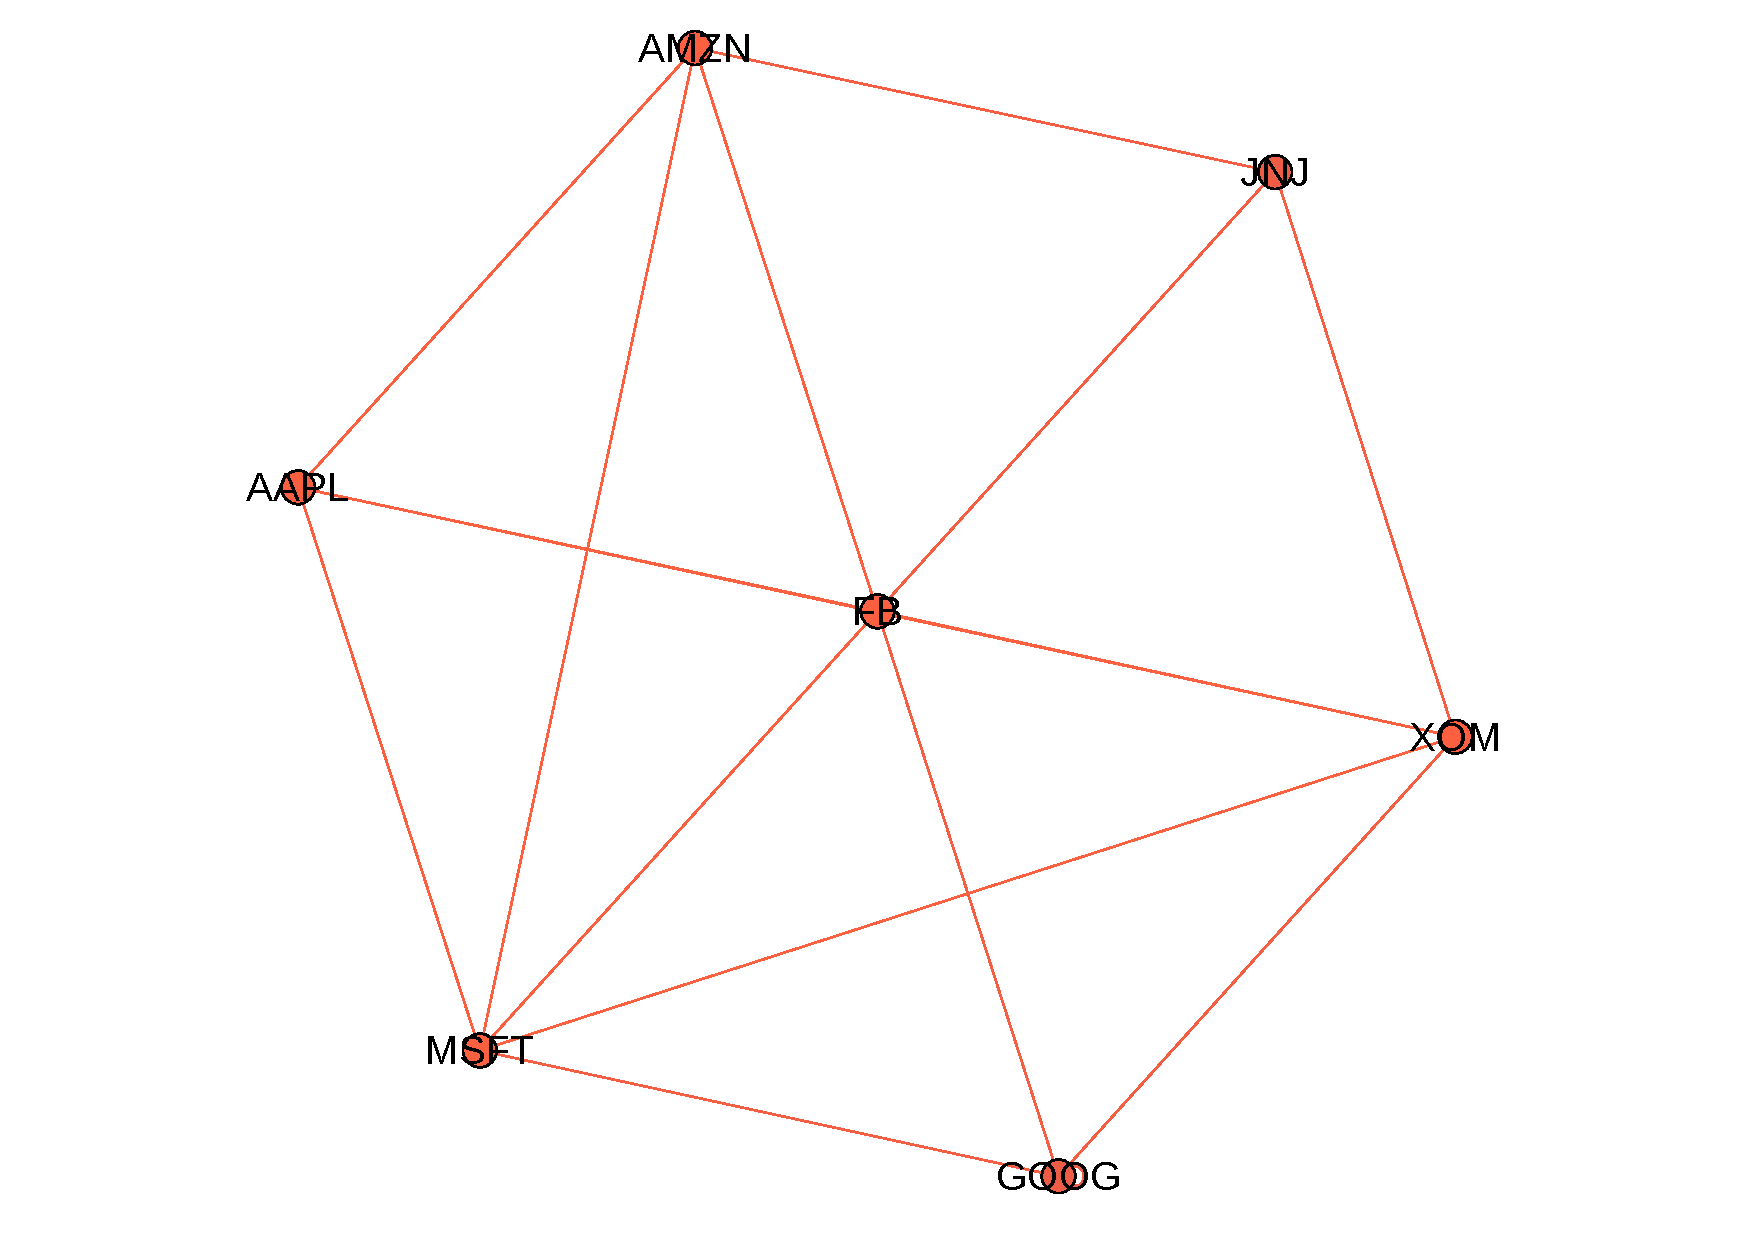
\includegraphics[width=\textwidth]{figures/Intro/ExampleNetwork.pdf}

      \caption{
      This figure contains an example of an undirected graph with 7 nodes and 16 edges. This graph is formed from randomly selecting stock symbol tickers from a set of tickers and forming connections randomly. The purpose of this data is solely to demonstrate the basics of network theory. The nodes are defined as circles and have ticker symbols overlaid on them. Edges are formed between nodes with lines between them. Since this is an undirected graph there is no directional information ergo no distinction as to whether one node is connected to another or vice-versa. The only information represented from an undirected graph is that they are connected. Lastly the amount of connections a node has is referred to as degree. So the node \(FB\) has 6 edges or a degree of 6.
      }
      \label{fig:ExampleNetwork}

  \end{figure*}

\begin{figure*}[!htb]
    \centering
     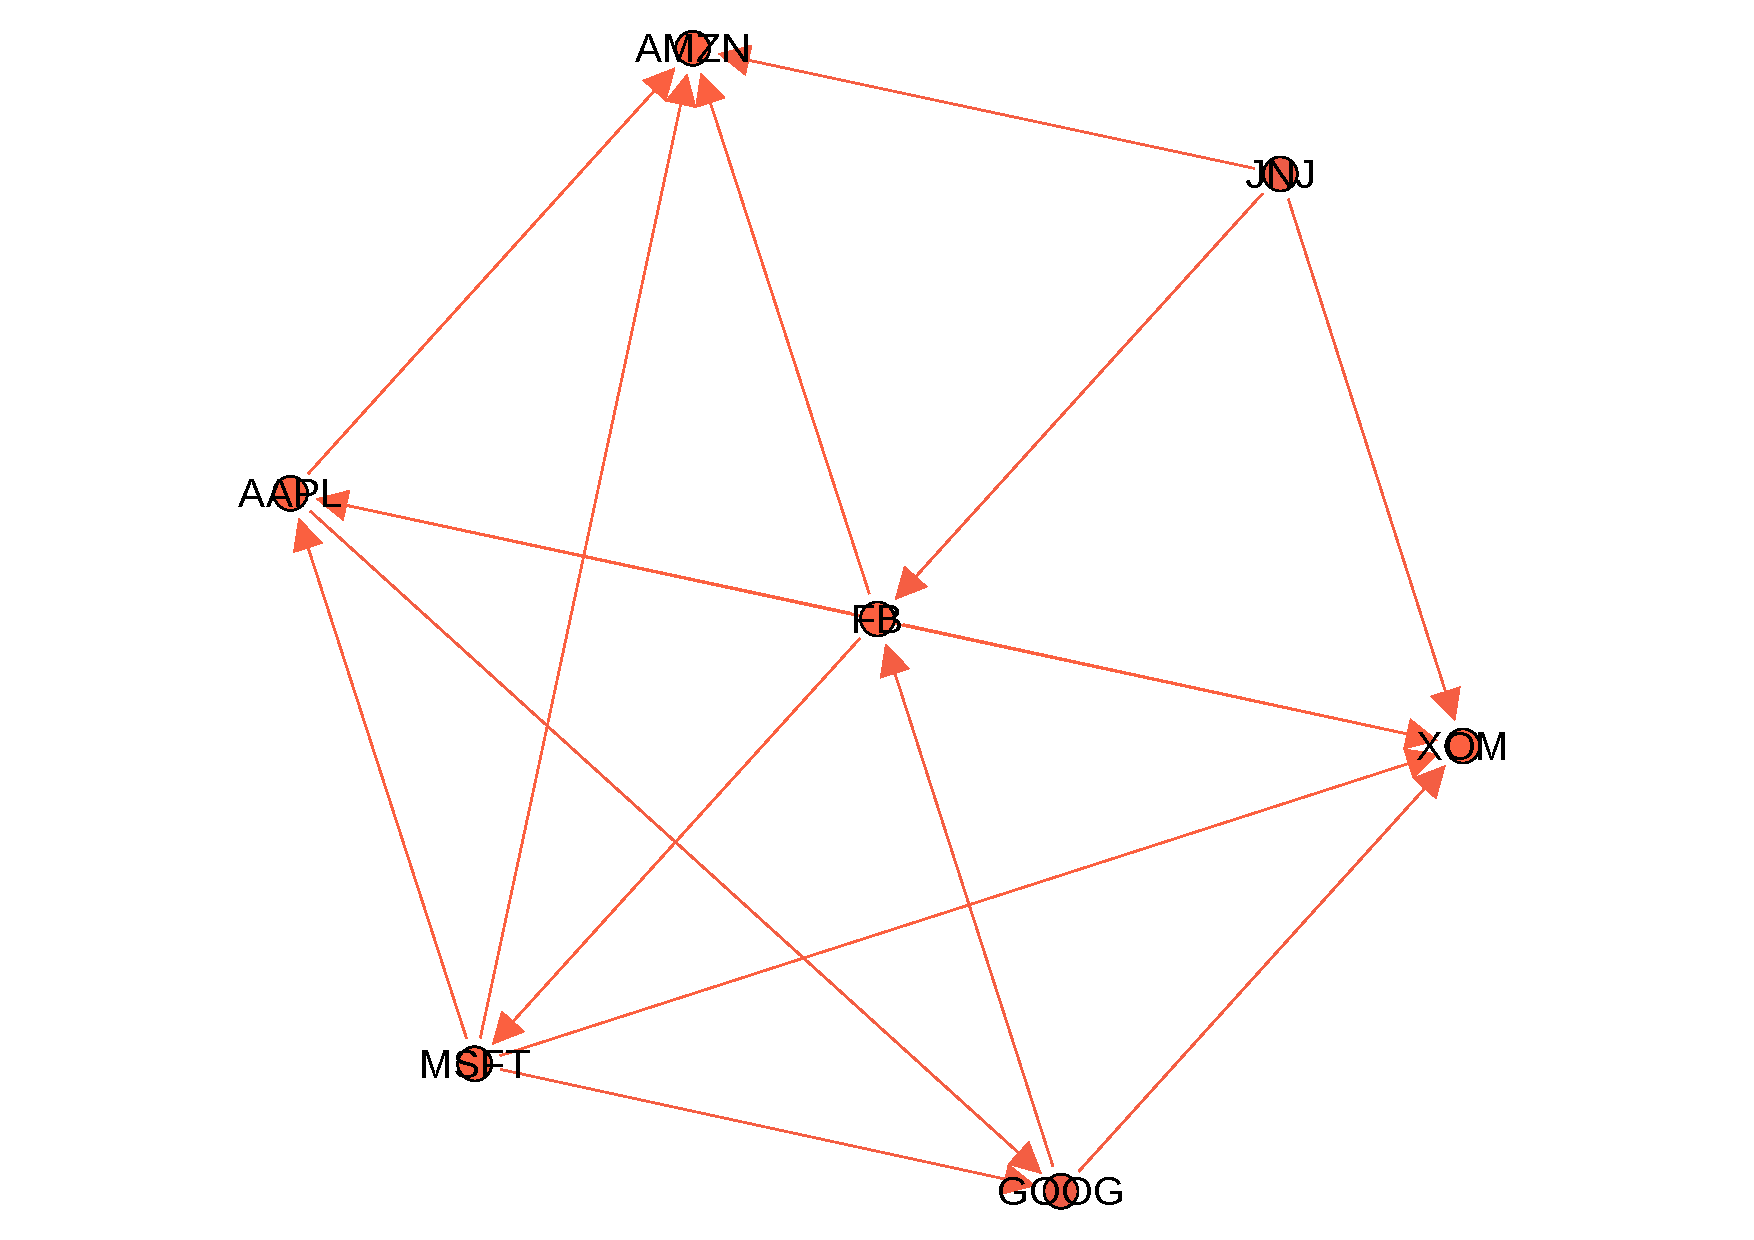
\includegraphics[width=\textwidth]{figures/Intro/ExampleNetworkDirected.pdf}
    \caption{
This graph is nearly identical to the graph in Figure \ref{fig:ExampleNetwork} except this graph is a directed network. This means that it contains directional information between the nodes. This directional information is communicated based on the position of the arrow in a line. For example, the node \(FB\) has an edge to \(MSFT\) however \(MSFT\) does not have an edge to \(FB\). The directional information allows other metrics to be used such as in-degree (which represents the amount of edges directed toward a node) and out-degree (which represents the amount of edges directed away from a node. In this example \(FB\) has an in-degree of 2, an out-degree of 4 and a degree of 6.
      }
	\label{fig:ExampleNetworkDirected}
\end{figure*}



  \begin{figure*}[!htb]
    \centering
      \centering
      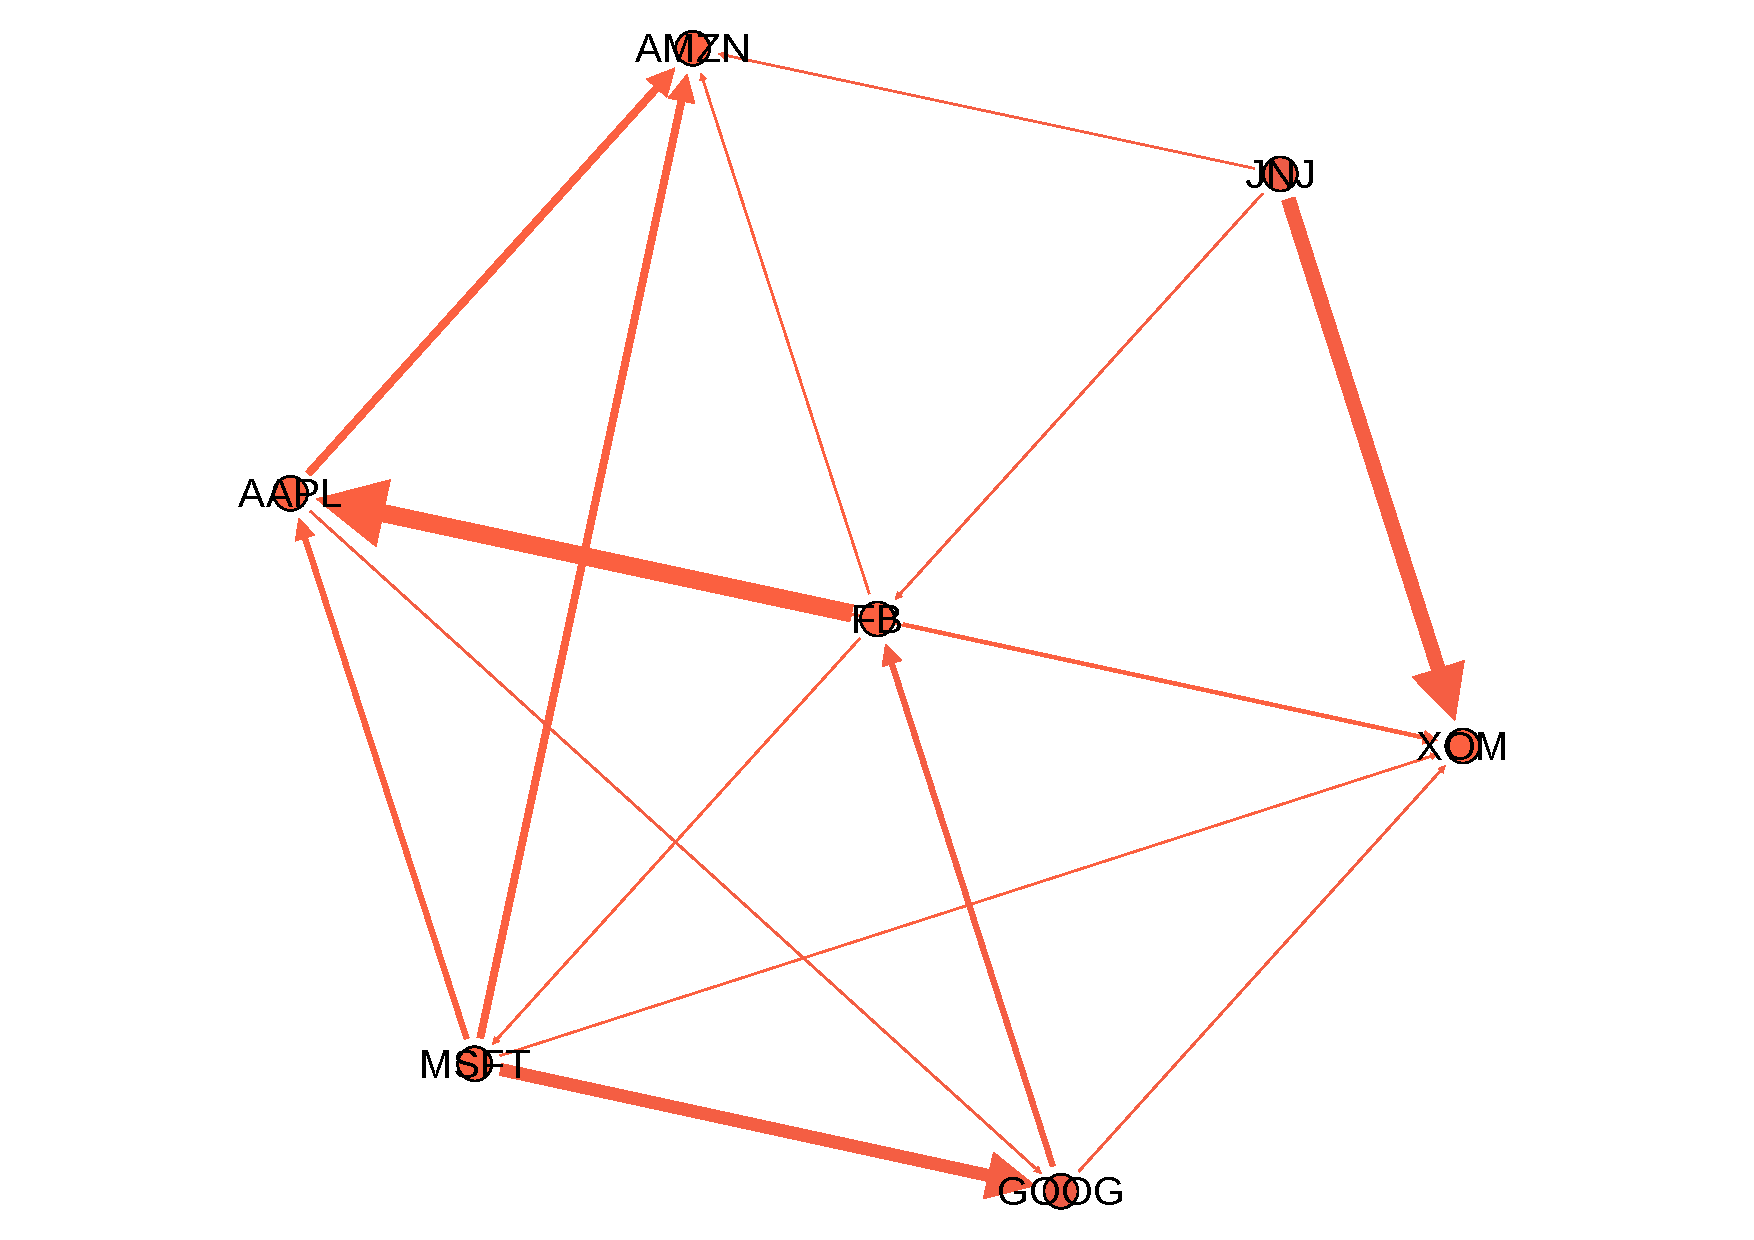
\includegraphics[width=\textwidth]{figures/Intro/ExampleNetworkDirectedWeighted.pdf}
      \caption{A nearly identical graph to the graph in Figure \ref{fig:ExampleNetworkDirected}. This directed graph contains weighted edges where a thick edge represents a high weight value (or strong connection). The smaller the edge weight value the thinner the edge will be.  Here \(FB\) has a strong connection to \(AAPL\) whereas \(FB\) has a weak connection to \(AMZN\).}
      \label{fig:ExampleNetworkDirectedWeighted}
    
  \end{figure*}

\begin{figure*}[!htb]
    \centering
      \centering
      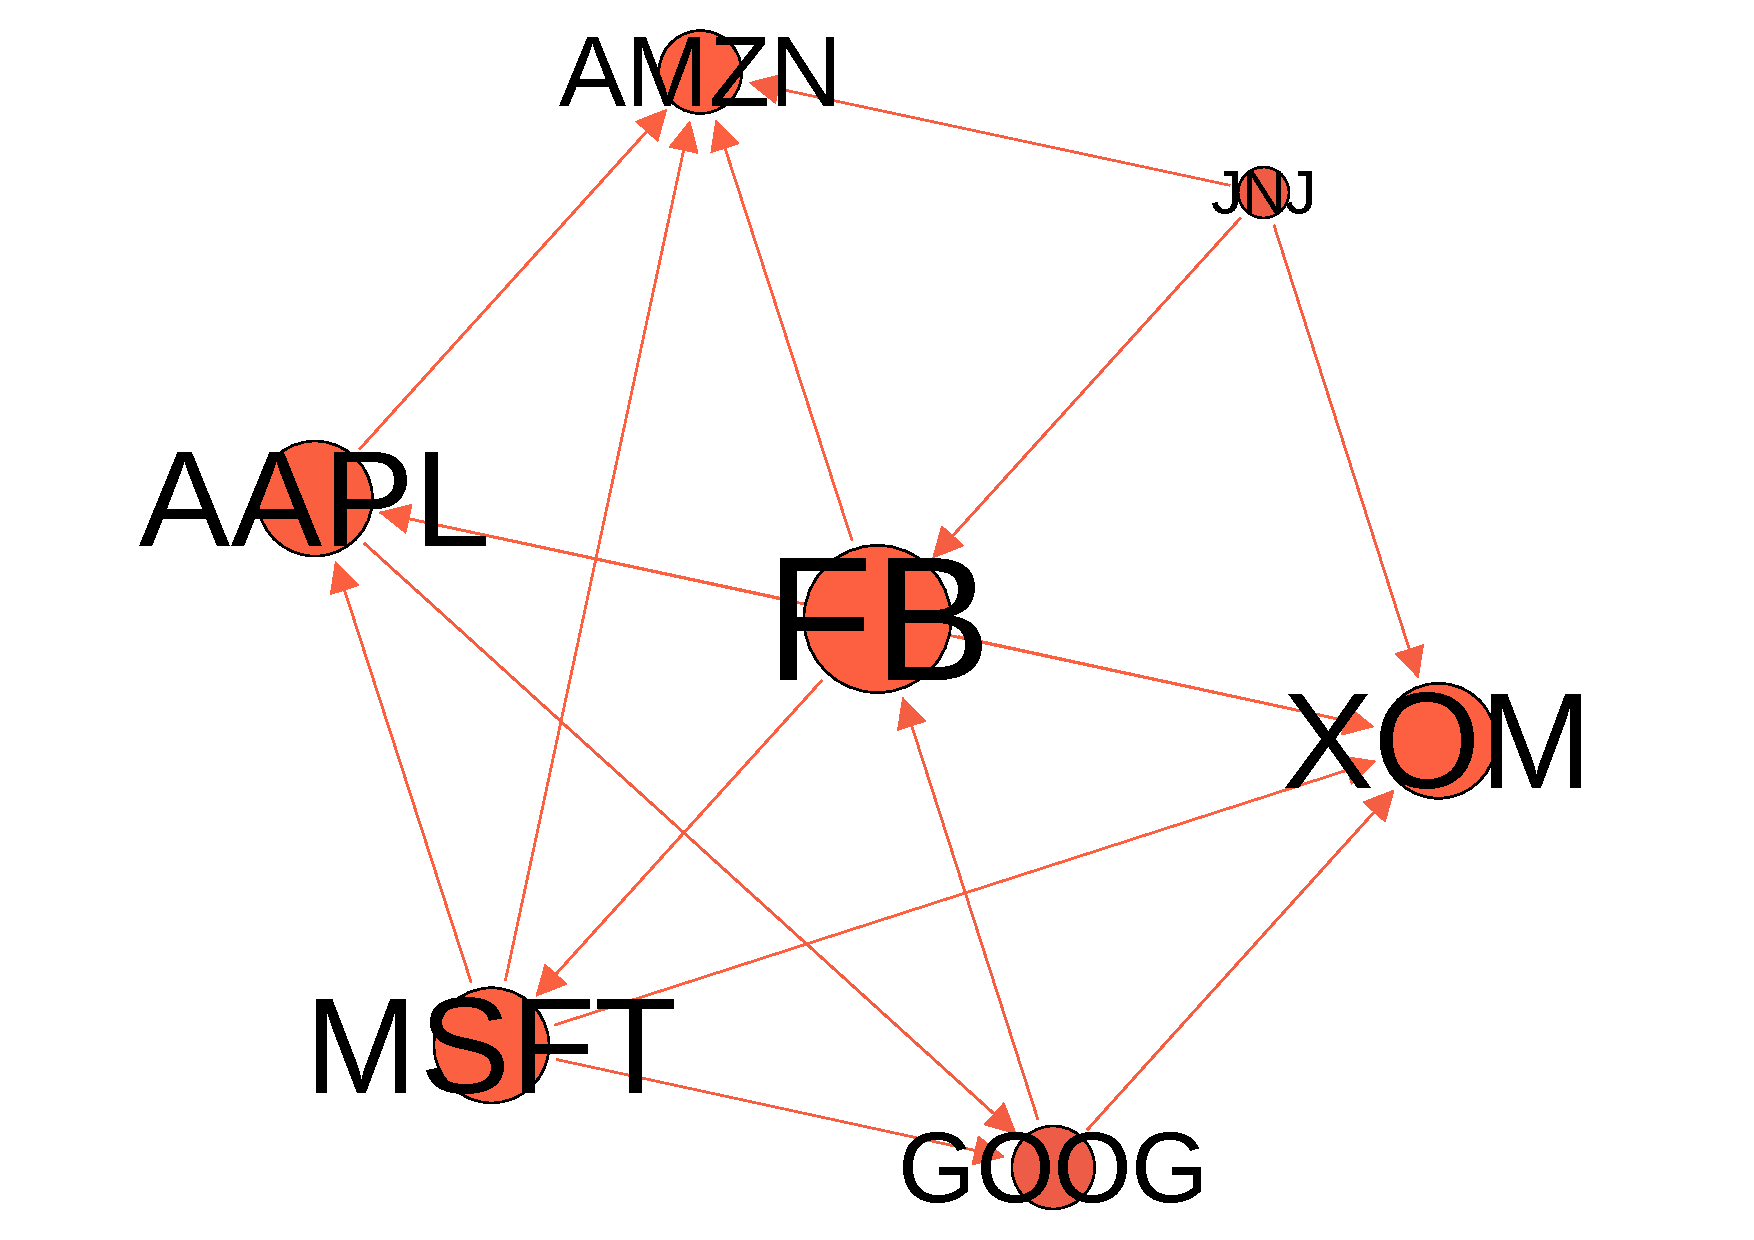
\includegraphics[width=\textwidth]{figures/Intro/ExampleNetworkDegree.pdf}
    \caption{
      A nearly identical graph to the graph in Figure \ref{fig:ExampleNetworkDirected}. Here the node sizes are scaled based on the degree. The higher the degree the larger the node size and consequently the smaller the degree the smaller the node size.
      }
      \label{fig:ExampleNetworkDegree}
  \end{figure*}


\begin{table}[htbp]
\begin{center}
    \begin{tabular}{|p{2cm}|p{1.5cm}|p{1.5cm}|p{1.5cm}|p{1.5cm}|p{1.5cm}|p{1.5cm}|p{1.5cm}|  }
        \hline
         & MSFT & AAPL & AMZN & FB & JNJ &  GOOG & XOM\\
        \hline
        MSFT  & 0 & 1 & 1 & 1  & 0 & 1 & 1 \\
        \hline
        AAPL & 1& 0 & 1 & 1 & 0 & 1 & 1 \\
        \hline
        AMZN & 1 & 1 & 0 & 1 & 1  & 0 & 0 \\
        \hline
        FB & 1 & 1 & 1 & 0  & 1 & 1 & 1 \\
        \hline
        JNJ & 0 & 0 & 1 & 1 & 0 & 0 & 0  \\ 
        \hline
        GOOG & 1 & 1 & 0 & 1 & 0 & 0 & 1 \\
        \hline
        XOM & 1 & 1 & 0 & 1 & 0 & 1 & 0  \\
        \hline
    \end{tabular}
\end{center}
\caption{ 
      This table contains an example of simulated data. This table was formed from randomly selecting stock symbol tickers from a set of tickers. The purpose of this data is solely to demonstrate the basics of network theory. Here the columns and row indicies belong to the selected tickers. The values contain either a 1 to represent if there is a connection between the ticker at a particular row index \(i\)  and the ticker of a particular column \(j\) or a 0 if there is no connection.
}

\label{tab:ExampleTable}
\end{table}

\begin{figure*}[!htb]
    \centering
      \centering
      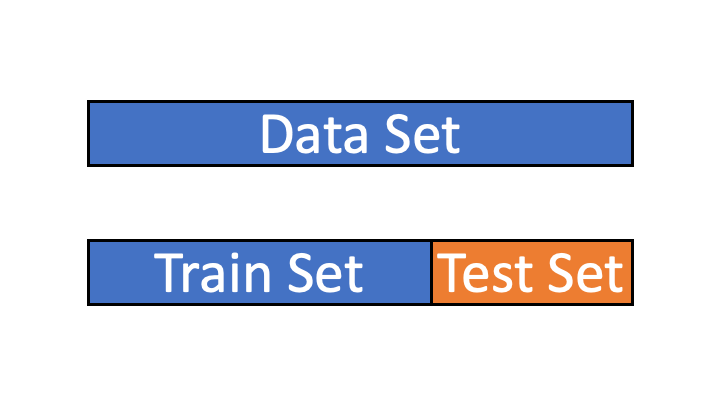
\includegraphics[width=\textwidth]{figures/ppt/TrainTestSplit.png}
    \caption{
      This figure shows how a data set can be partitioned for a supervised machine learning paradigm. The ``Data Set" is partitioned into 2 unequal sets with the``Train Set" having more data assigned to it than the ``Test Set". The ``Train Set" and ``Test Set" ratios can vary and is typically determined by the practitioner. There are many ways to partition the data for the train and test sets. For example the dataset can be partitioned sequentially from the data, or form partitions based on the data being randomly sampled.
      }
\label{fig:TrainTestSplit}

  \end{figure*}


\begin{figure*}[!htb]
    \centering
      \centering
      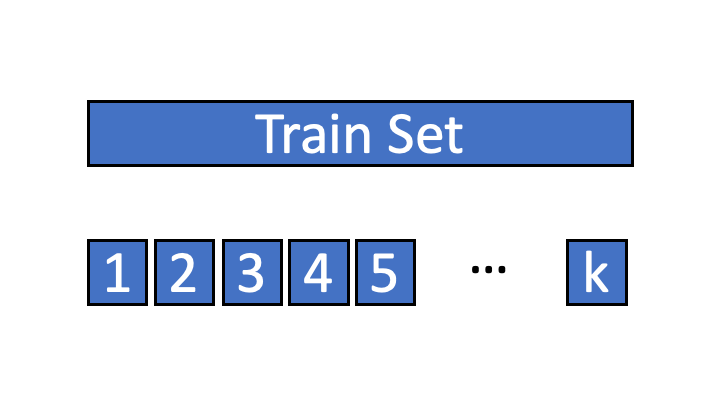
\includegraphics[width=\textwidth]{figures/ppt/KFoldValidation.png}
    \caption{
	``Train Set" here represents ``Train Set" in Figure \ref{fig:TrainTestSplit}. In this figure the data is split into \(k\) folds. How the \(k\) folds are created can vary. A common technique is to randomly divide the ``Train Set" observations into \(k\) equal folds.
      }
     \label{fig:KFoldValidation}
  \end{figure*}

\begin{figure*}[!htb]
    \centering
      \centering
      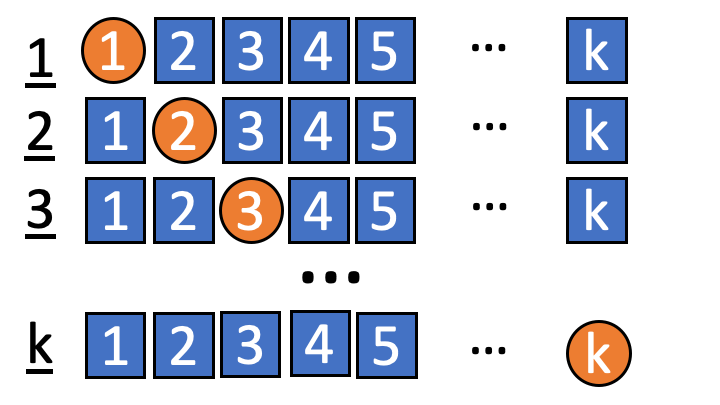
\includegraphics[width=\textwidth]{figures/ppt/KFoldValidationExplain.png}
     
    
    \caption{
	This figure breaks down how \(k\)-Fold Cross Validation works. These folds are created from ``Train Set" in Figure \ref{fig:KFoldValidation}. For the first iteration (where you see 1 underlined), the 1st fold (circle labeled 1) is used to assess the models ability and the remaining folds (squares) are used to train the model. The 2nd iteration follows the same procedure as the 1st except only the 2nd fold is withheld and the other folds are used. This repeats \(k\) times.
      }
\label{fig:KFoldValidationExplain}
  \end{figure*}


\begin{figure*}[!htb]
    \centering
      \centering
      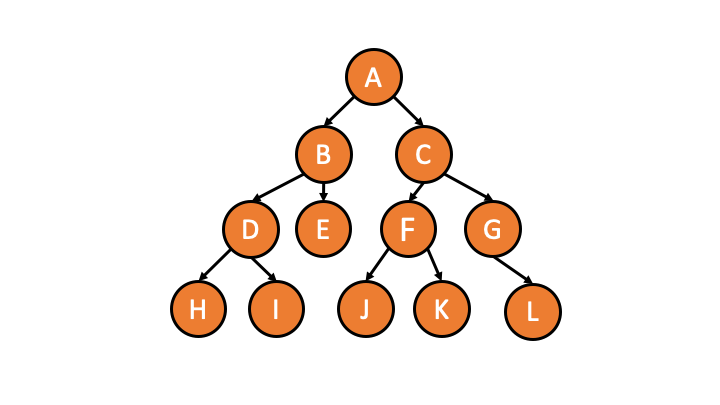
\includegraphics[width=\textwidth]{figures/ppt/DecisionTree.png}

    \caption{
	This figure shows an example of a Decision Tree. This is essentially a graph with no cycles.  Each circle represents a node (the label of the node is a letter inside of the node) and the arrows represent directional edges (branches) to another node. Node \(A\) is the root node of this tree and is where the decision begins. Potential outcomes from the root node lead to different states that are represented in nodes \(B\) and \(C\). \(B\) and \(C\) are the children of \(A\).  Nodes \(B\) and \(C\) have children and their children has children. Nodes \(H, I, E, J, K,\) and \(L\) are the leaf nodes of this tree because they have no children.
      }
      \label{fig:DecisionTree}
  \end{figure*}

\clearpage
\bibliographystyle{plainnat}
\bibliography{thesisbib}
\include{2-related}
\include{3-model}
\include{4-predictions}

\chapter{Conclusions}

We conclude that graduate students like coffee.
% \iffalse
%<example>
% \fi
% \end{verbatim} \hrule \end{quote}
%
% \subsection{Reference Matter}
%
% \DescribeMacro{\appendix}
% To switch from the body of your thesis to the reference material
% at the end, you should use the standard \LaTeX\ |\appendix| command.
% In \pkg{uiucthesis2014}, there is also a starred version of this command
% that eliminates the lettering of the appendices (use if you have
% a single appendix). Note that if you use |\appendix*| along with
% the |[fancy]| option, you may want to put ``Appendix:'' at
% the beginning of the chapter title.
%
%
% \begin{quote} \hrule \begin{verbatim}
\appendix*

\chapter{Standard Machine Learning Language Supplemental Code}
\section{Iris Python Code}

This shows the code required to replicate the same actions of the SML \(Query\) in Figure \ref{fig:SML:IrisQuery}. It's important to note that detailed documentation is publicly available in \textsuperscript{\ref{lab:iris:git}}, the purpose of this figure is to highlight the level of complexity relative to a SML query.

\begin{lstlisting}[language=python]
import pandas as pd
import numpy as np

from sklearn.preprocessing import label_binarize
import sklearn.cross_validation as cv
from sklearn.multiclass import OneVsRestClassifier
from sklearn.svm import SVC
from sklearn.metrics import roc_curve, auc

import matplotlib.pyplot as plt
import seaborn as sns
names = ['sepal length(cm)', 'sepal width(cm)', 'petal length(cm)', 'petal width(cm)', 'species']
data = pd.read_csv('../data/iris.csv', names=names)

iris_classes = ['Iris-setosa', 'Iris-versicolor', 'Iris-virginica']
features = np.c_[data.drop('species',1).values]
labels = label_binarize(data['species'], classes=iris_classes)
n_classes = labels.shape[1]

x_train, x_test, y_train, y_test = cv.train_test_split(features, labels, test_size=0.25)
svm = OneVsRestClassifier(SVC(kernel='linear', probability=True))
l = svm.fit(x_train, y_train)
predict_score = model.decision_function(x_test)
test_set_results = model.score(x_test, y_test) * 100
print ('SVM Prediction Accuracy = {0:6.2f}%'.format(test_set_results) )
 fpr = dict()
tpr = dict()
roc_auc = dict()

for i in range(n_classes):
fpr[i], tpr[i], _ = roc_curve(y_test[:, i], predict_score[:, i])
roc_auc[i] = auc(fpr[i], tpr[i])
plt.rcParams['figure.figsize']=(12,12)
# Class Info
columns = [0,1,2,3]
cmap_class = ['Purples_r', 'Greens_r', 'Oranges_r', 'Greys_r' ]
color_class1D = ['purple', 'darkgreen', 'orange', 'grey']
column_headers =  data.columns.values.tolist() # Grab headers from df
column_headers = [column_headers[x] for x in columns] # Map headers to indices selected

label = 'species'
fig, ax = plt.subplots(len(columns), len(columns))
for ic, cc, cc1D in zip(iris_classes, cmap_class, color_class1D): 
  iris_class_data = data.loc[data.species == ic] # sep class
   
  #Generate kde plot matrix for class
  for col1, i in enumerate(columns):
      for col2, j in enumerate(columns):
          if i == j:
              sns.kdeplot(iris_class_data[iris_class_data.columns[col1]], ax=ax[col1][col2], color=cc1D, shade=True, legend=False)
          else:
              sns.kdeplot( iris_class_data[iris_class_data.columns[col1]], iris_class_data[iris_class_data.columns[col2]], ax=ax[col1][col2], cmap=cc)    
          # Formatting
          if j == 0:
              ax[i,j].set_xticklabels([])
              ax[i,j].set_ylabel(column_headers[i])
              ax[i,j].set_xlabel('')
              if i == len(columns)-1:
                  ax[i,j].set_xlabel(column_headers[j])
          elif i == len(columns)-1:
              ax[i,j].tick_params(axis='y', which='major', bottom='off')
              ax[i,j].set_yticklabels([])
              ax[i,j].set_xlabel(column_headers[j])
              ax[i,j].set_ylabel('')                
          else:
              ax[i,j].set_xticklabels([])
              ax[i,j].set_xlabel('')
              
              ax[i,j].set_yticklabels([])
              ax[i,j].set_ylabel('')
  
plt.show()
plt.close()
\end{lstlisting}

\clearpage

\section{Auto-MPG Python Code}
This shows the code required to replicate the same actions of the SML \(Query\) in Figure \ref{fig:SML:AutoMPGQuery}. It's important to note that detailed documentation is publicly available in \textsuperscript{\ref{lab:SML:AUTO}}, the purpose of this figure is to highlight the level of complexity relative to a SML query.
\begin{lstlisting}[language=python]
import pandas as pd
import numpy as np

import matplotlib.pyplot as plt
from sklearn import linear_model
from sklearn.cross_validation import train_test_split
from sklearn.learning_curve import learning_curve, validation_curve

import matplotlib.pyplot as plt
import seaborn as sns

plt.rcParams['figure.figsize']=(12,12)
sns.set()
 
names = ['mpg', 'cylinders', 'displacement', 'horsepower', 'weight', 'acceleration', 'model_year', 'origin', 'car_name']
 
#load dataset
data = pd.read_csv('../data/auto-mpg.csv', sep = '\s+', header = None, names = names)
data_clean=data.applymap(lambda x: np.nan if x == '?' else x).dropna()
X = data_clean[['cylinders', 'displacement', 'horsepower', 'weight', 'acceleration', 'model_year', "origin"]]
#Select target column
y = data_clean['mpg']
#Split data into training and testing sets
X_train, X_test, y_train, y_test = train_test_split(X, y, train_size=0.8, test_size=0.2)

# Define and train  linear regression model
estimator = linear_model.LinearRegression()# Generate Learning Cures
train_sizes, train_scores, test_scores = learning_curve(estimator, X_train, y_train) 
# Train Linear Regression Model
estimator.fit(X_train, y_train)# Generate Validation Curves
param_range = np.arange(0, 5)

v_train_scores, v_test_scores = validation_curve(estimator, X_test, y_test, param_name='normalize', param_range=param_range)

score = estimator.score(X_test, y_test)
print('Accuracy :', score)
g = sns.PairGrid(data_clean, palette='PuOr_r')
g = g.map_diag(sns.kdeplot, shade=True) # can't add color arg...
 
g = g.map_upper(sns.kdeplot, cmap='PuOr_r')
g = g.map_lower(sns.kdeplot, cmap='PuOr_r')
 
plt.show()
plt.close()
 
color_pal = ['purple', 'dark green', 'orange', 'grey'] # For 1-D KDE
cmap_pal = ['PuOr_r'] # For 2-D KDE
classes = [] # May not have a class for categories

column_headers =  data_clean.columns.values.tolist() # Grab headers from df
column_headers = [column_headers[x] for x in columns] # Map headers to indices selected
 
fig, ax = plt.subplots(len(columns), len(columns))
if not classes:
  for col1, i in enumerate(columns):
      for col2, j in enumerate(columns):
          if i == j:
              sns.kdeplot(data_clean[data_clean.columns[col1]], ax=ax[col1][col2], color=color_pal[0], shade=True, legend=False)
          else:
              sns.kdeplot( data_clean[data_clean.columns[col1]], data_clean[data_clean.columns[col2]], ax=ax[col1][col2], cmap=cmap_pal[0])

           # Formatting
           if j == 0:
               ax[i,j].set_xticklabels([])
               ax[i,j].set_ylabel(column_headers[i])
               ax[i,j].set_xlabel('')
                if i == len(columns)-1:
                   ax[i,j].set_xlabel(column_headers[j])
            elif i == len(columns)-1:
                ax[i,j].tick_params(axis='y', which='major', bottom='off')
                ax[i,j].set_yticklabels([])
                ax[i,j].set_xlabel(column_headers[j])
                ax[i,j].set_ylabel('')            
            else:
                ax[i,j].set_xticklabels([])
                ax[i,j].set_xlabel('')            
                ax[i,j].set_yticklabels([])
                ax[i,j].set_ylabel('')
plt.show()
plt.close()
 
plt.figure()
plt.xlabel("Validation examples")
plt.ylabel("Score")
 
v_train_scores_mean = np.mean(v_train_scores, axis=1)
v_train_scores_std = np.std(v_train_scores, axis=1)
v_test_scores_mean = np.mean(v_test_scores, axis=1)
v_test_scores_std = np.std(v_test_scores, axis=1)
 
plt.fill_between(param_range, v_train_scores_mean - v_train_scores_std, v_train_scores_mean + v_train_scores_std, alpha=0.1, color="orange")
plt.fill_between(param_range, v_test_scores_mean - v_test_scores_std, v_test_scores_mean + v_test_scores_std, alpha=0.1, color="purple")plt.plot(param_range, v_train_scores_mean, 'o-', color="orange", label="Training score")
 
plt.plot(param_range, v_test_scores_mean, 'o-', color="purple", label="Cross-validation score")
 
plt.legend(loc="best")
plt.show()
plt.close()
\end{lstlisting}
% \end{verbatim} \hrule \end{quote}
% \iffalse
%<example>
% \fi
%
% \subsection{Back Matter}
%
% \DescribeMacro{\backmatter}
% The last few chapters in your thesis should not have chapter
% numbers, but should be listed in the Table of Contents.
% These chapters include the Bibliography and the Index.  \LaTeX's
% |\backmatter| command accomplishes this.
%
% \DescribeMacro{\bibliography}
% Use the standard \LaTeX\ bibliography commands to
% create your bibliography. Most people will use Bib\TeX\ to do this.
% (See \cite{Lamport}). For those in the sciences, you may want to
% check out the \pkg{cite} package (it's pretty standard), which
% will produce numerical citations that are sorted and compressed.
% You can also use the \pkg{natbib} package. Both of these packages
% can do either bracketed citations or superscript citations.
%
% \begin{quote} \hrule \begin{verbatim}
\backmatter

\bibliographystyle{apalike}
\bibliography{thesisbib}

\end{document}
% \end{verbatim} \hrule \end{quote}
%
% \iffalse
%</example>
% \fi
%
% \section{User Customization}
%
% \DescribeMacro{\draftheader}
% If you don't like the header that the the |[draftthesis]| option
% creates, you can redefine the |\draftheader| command so that it
% produces whatever text you want.
%
% \DescribeMacro{\thesisspacing}
% The \pkg{uiucthesis2014} class loads \pkg{setspace} for the
% line spacing commands.  See the documentation in that package
% for more information on the commands it provides.
% By default, \pkg{uiucthesis2014} uses one and a half line spacing,
% or double spacing if the |[fullpage]| option is specified.
% If you're unhappy with that, you can override it by redefining the
% |\thesisspacing| command.
%
% \DescribeMacro{\nocopyrightpage}
% Unless the |[draftthesis]| option is used, a page with the copyright notice
% is printed before the title page. If you don't want this page to
% appear, even in the final version, put the |\nocopyrightpage| macro
% somewhere in the preamble.
%
% \DescribeMacro{\toclabels}
% Some departments require the Table of Contents, List of Tables and
% List of Figures to have a ``Page'' heading over the page numbers
% on the first page. This can be accomplished by putting the |\toclabels|
% command somewhere before the |\tableofcontents| command. (NOTE: if you put
% the |\tableofcontents| command in a separate file that you |\include| in
% the main file, the |\toclabels| command must also be in that file.)
%
% \DescribeMacro{\chaptertitlefont}
% \DescribeMacro{\sectiontitlefont}
% \DescribeMacro{\subsectiontitlefont}
% \DescribeMacro{\subsubsectiontitlefont}
% These macros contain the font declarations for the corresponding sectioning
% levels and can be redefined to suit your aesthetic desires. Use
% |\renewcommand| to do this in the preamble.
%
% \DescribeMacro{\chapternumberfont}
% The |\chapternumberfont| macro is really most applicable when the |[fancy]| option is used. It
% specifies the font declaration used for the chapter number set in the left
% margin next to the title. Otherwise it specifies the font used to print
% the words ``Chapter \#'' at the top of each chapter's opening page. Use
% |\renewcommand| to redefine this macro in the preamble.
%
% \DescribeMacro{\chaptertitleheight}
% |\chaptertitleheight| is the amount of space allotted for the chapter title at the top
% of the page. You can redefine it using |\setlength| in the preamble.
%
% \DescribeMacro{\bibname}
% |\bibname| is a standard \LaTeX\ macro that contains the title of the reference
% section at the end of your thesis; ``References'' by default. Use
% |\renewcommand| to redefine it in the preamble.
%
% \DescribeMacro{\abstractname}
% Like above, but for the abstract. By default, ``Abstract''.
%
% \DescribeMacro{other "name"s}
% Similarly, the titles for the Table of Contents, List of Figures, and List of Tables
% are stored in the macros |\contentsname|, |\listfigurename|, and |\listtablename|,
% respectively. Their default values are the names in the previous sentence. There are
% also the macros |\chaptername|, |\appendixname|, |\indexname|, |\partname|,
% |\tablename|, and |\figurename| that contain the appellations for chapter and appendix
% headings (not applicable with the |[fancy]| option), the index, parts, tables, and figures.
% Their default values are Chapter, Appendix, Index, Part, Table, and Figure, respectively.
% All of these macros can
% be redefined in the preamble with |\renewcommand|.  These macros are all part of
% the standard \LaTeX\ formalism, they are just included here for the reader's convenience.
% For example, some departments require chapter headings to be in all caps, which can
% be done by changing the |\chaptername| macro to be CHAPTER.
%
% \DescribeMacro{\note}
% This command inserts a marginal note just like |\marginpar| with two distinctions:
% First, the note is single-spaced in a smaller type for compactness.
% Second, it is only printed when
% the |[draftthesis]| option is used. Since marginal notes are not allowed in the final
% draft, the |\note| command is recommended over the |\marginpar| command.
%
% \section{Backwards Compatibility}
%
% Compatibility with previous versions of \pkg{uiucthesis2014} are supported. Previously it
% was implemented as a package rather than a class, in which case you opened the document
% with:
% \begin{quote} \hrule \begin{verbatim}
% \documentclass[oneside,...]{book}
% \usepackage[...]{uiucthesis2014}
% \end{verbatim} \hrule \end{quote}
% To provide backwards-compatibility, a style file is provided that has the same functionality
% of the class file described herein. Similarly, (really) old versions of \pkg{uiucthesis2014}
% used the \env{preliminary} and \env{thesis} environments, which are now deprecated
% but backwards-compatibility support is still provided.
%
% \section{Other Issues}
%
% \subsection{Paper Size and PDF Files}
%
% The default paper size for most \LaTeX\ distributions is A4, which is slightly different
% the 8.5 x 11 size for letter paper in the U.S\@. The Graduate College requires theses
% to be letter paper size.  In addition, many departments want soft copies of the thesis
% in PDF format. Unfortunately, the program used to convert the dvi file to PDF format
% (|dvipdfm| on my computer, which is a Windows machine with Mik\TeX installed on it)
% often produces PDF files in A4 format, even if |letterpaper|
% is specifically specified in the your \TeX source file. If you're having this problem,
% either run the PDF conversion utility from the command line with the right flag ---
% for example, |dvipdfm -p letter| on my computer --- or change the default paper size in
% the config file for your PDF conversion utility, which will then fix this problem
% permanently.  On my computer, this can be done by going to the |dvipdfm\config|
% subdirectory off of the main \TeX installation directory (usually |C:\texmf|). In this
% directory is a file called |config| that has a line for the default paper size.
%
% \subsection{Reference Lists at the Chapter Level}
%
% The \pkg{cite} package includes a style file \pkg{chapterbib.sty} that can be used
% to do a list of references for each chapter instead of just one big list at the
% end of the thesis.  I've not used this style before so you're on your own if you
% want to do this, but I think it is rather straightforward\ldots.
%
% \StopEventually{%
%   \begin{thebibliography}{9}
%     \bibitem{Handbook}
%     \emph{Handbook for Graduate Students Preparing to Deposit}.
%     \newblock Graduate College, University of Illinois at
%     Urbana-Champaign, 2004
%
%     \bibitem{thesisweb}
%      \emph{Grad College webpage with thesis requirements}.
%      \newblock |http://www.grad.illinois.edu/graduate-college-thesis-requirements|
%
%     \bibitem{Lamport}
%     Leslie Lamport.
%     \newblock \emph{\LaTeX: A Document Preparation System}.
%     \newblock Addison-Wesley, 1994.
%   \end{thebibliography}
% }
%
% \section{Implementation}
%
% This section shows the implementation of the \pkg{uiucthesis2014} class.
% Unless you are interested in the details of how \pkg{uiucthesis2014} works,
% you probably don't need to read it.
%
% \iffalse
%<*class|package>
\RequirePackage{setspace}
% \fi
%
% \subsection{Compatibility}
%
% Provide compatibililty with older versions of \LaTeX.
% \begin{macro}{\@ifundefined}
%    \begin{macrocode}
\expandafter\ifx\csname @ifundefined\endcsname\relax
  \def\@ifundefined#1{%
    \expandafter\ifx\csname#1\endcsname\relax
      \expandafter\@firstoftwo
    \else
      \expandafter\@secondoftwo
    \fi}
\fi
%    \end{macrocode}
% \end{macro}
%
% \begin{macro}{\MakeUppercase}
%    \begin{macrocode}
\@ifundefined{MakeUppercase}{\let\MakeUppercase=\uppercase}{}
%    \end{macrocode}
% \end{macro}
%
% \subsection{Option Processing}
%
%    \begin{macrocode}
\newif\if@thesisdraft \@thesisdraftfalse
\newif\if@thesisfancy \@thesisfancyfalse
\newif\if@fullpage \@fullpagefalse
\newif\if@largecaps \@largecapsfalse
\newif\if@proquest \@proquestfalse
\newif\if@edeposit \@edepositfalse
\newif\if@thesisoffcenter \@thesisoffcenterfalse
\newif\if@centerchapter \@centerchapterfalse
%    \end{macrocode}
%
%    \begin{macrocode}
\DeclareOption{draftthesis}{\@thesisdrafttrue}
\DeclareOption{fancy}{\@thesisfancytrue}
\DeclareOption{fullpage}{\@fullpagetrue}
\DeclareOption{proquest}{\@proquesttrue}
\DeclareOption{toclabels}{\AtBeginDocument{\toclabels}}
\DeclareOption{edeposit}{\@edeposittrue}
\DeclareOption{offcenter}{\@thesisoffcentertrue}
\DeclareOption{centerchapter}{\@centerchaptertrue}
%    \end{macrocode}
%
% The |[largecaps]| option causes the title and author's name to
% be use a ``large caps'' font on the title page.  Otherwise,
% \pkg{uiucthesis2014} just converts them to uppercase and uses the
% normal fonts.  The difference is that the spacing between the
% characters in the large caps font is tuned for setting type in all caps.
%
% The large caps font is \emph{not a standard font}, and so it will not exist
% unless you have installed it.
%
%    \begin{macrocode}
\DeclareOption{largecaps}{\@largecapstrue}
%    \end{macrocode}
%
% Load the \pkg{book} class with the |[oneside]| and |[letterpaper]| options
%
%    \begin{macrocode}
%<class>\DeclareOption*{\PassOptionsToClass{\CurrentOption}{book}}
%<class>\PassOptionsToClass{letterpaper,oneside}{book}
\ProcessOptions
%<class>\LoadClass{book}
%    \end{macrocode}
%
% If the |[proquest]| option is used, turn off output to auxiliary files so
% that the thesis doesn't have to be recompiled again to get all the references
% correct. Also double-space the ProQuest abstract and use the full page.
%
%    \begin{macrocode}
\if@proquest
    \nofiles    % don't overwrite the .aux files
    \def\makeindex{}
    \@thesisfancyfalse
    \@fullpagetrue
\fi
%    \end{macrocode}
%
% If the |[draftthesis]| option was specified, define the |\draftheader| macro.
%
%    \begin{macrocode}
\if@thesisdraft
  \newcount\timehh\newcount\timemm
  \timehh=\time \divide\timehh by 60
  \timemm=\time \count255=\timehh \multiply\count255 by -60
    \advance\timemm by \count255
  \def\draftheader{\slshape Draft of \today\ at
  \ifnum\timehh<10 0\fi\number\timehh\,:\,\ifnum\timemm<10 0\fi\number\timemm}%
\fi
%    \end{macrocode}
%
% Define the |\toclabels| command which prints the headings in the Table of Contents,
% List of Figures and List of Tables.
%
%    \begin{macrocode}
\newcommand{\toclabels}{%
    \addtocontents{toc}{\vspace*{-\baselineskip}\hfill Page\endgraf}%
    \addtocontents{lof}{\vspace*{-\baselineskip}~Figure\hfill Page\endgraf}%
    \addtocontents{lot}{\vspace*{-\baselineskip}~Table\hfill Page\endgraf}}
%    \end{macrocode}
%
% \subsection{Title Page}
%
% \begin{macro}{\title}
% \begin{macro}{\author}
% Override the standard definitions of |\title| and |\author| to also
% define uppercased versions.
%    \begin{macrocode}
\def\@mkuptitle#1{\gdef\@Utitle{#1}}
\def\title#1{\gdef\@title{#1}\MakeUppercase{\protect\@mkuptitle{#1}}}
\def\@mkupauthor#1{\gdef\@Uauthor{#1}}
\def\author#1{\gdef\@author{#1}\MakeUppercase{\protect\@mkupauthor{#1}}}
%    \end{macrocode}
% \end{macro}
% \end{macro}
%
% \begin{macro}{\phdthesis}
% \begin{macro}{\msthesis}
% \begin{macro}{\otherdoctorate}
% \begin{macro}{\othermasters}
% \begin{macro}{\department}
% \begin{macro}{\college}
% \begin{macro}{\schools}
% \begin{macro}{\degreeyear}
% \begin{macro}{\committee}
% \begin{macro}{\volume}
% Macros to set title page elements.
%    \begin{macrocode}
\def\phdthesis{\def\@degree{Doctor of Philosophy}
    \def\degree{Ph.D.}
    \def\@thesisname{DISSERTATION}
    \def\@committeename{Doctoral Committee:}
    }
\def\msthesis{\def\@degree{Master of Science}
    \def\degree{M.S.}
    \def\@thesisname{THESIS}
    \def\@committeename{Master's Committee:}
    }
\newcommand{\otherdoctorate}[2]{\def\@degree{#1}
    \def\degree{#2}
    \def\@thesisname{DISSERTATION}
    \def\@committeename{Doctoral Committee:}
    }
\newcommand{\othermasters}[2]{\def\@degree{#1}
    \def\degree{#2}
    \def\@thesisname{THESIS}
    \def\@committeename{Master's Committee:}
    }
\def\department#1{\def\@dept{#1}}
\def\college#1{\def\@college{#1}}
\def\schools#1{\def\@schools{#1}}
\def\degreeyear#1{\def\@degreeyear{#1}}
\newcommand{\committee}[1]{\gdef\@committee{#1}}
\newcommand*{\volume}[1]{\gdef\thesis@volume{VOLUME~#1}}
\newcommand*{\thesis@volume}{}
\if@edeposit
  \gdef\@committee{%
%<class>    \ClassError{uiucthesis2014}{A committee must be specified for e-deposit dissertations.}%
%<package>    \PackageError{uiucthesis2014}{A committee must be specified for e-deposit dissertations.}%
    {Use \protect\committee\space with members separated by \protect\\'s.}}
\fi
%    \end{macrocode}
% \end{macro}
% \end{macro}
% \end{macro}
% \end{macro}
% \end{macro}
% \end{macro}
% \end{macro}
% \end{macro}
% \end{macro}
% \end{macro}
%
% \begin{macro}{\copyrightnotice}
% Define the copyright notice as a macro so that the user
% can change it if desired.
%    \begin{macrocode}
\def\copyrightnotice{\copyright~\@degreeyear~by \@author. All rights reserved.}
%    \end{macrocode}
% \end{macro}
% \begin{macro}{\nocopyrightpage}
% The printing of the copyright page can also be turned off with the
% |\nocopyrightpage| command (must come before |\maketitle|):
%    \begin{macrocode}
\newif\if@thesiscrpage \@thesiscrpagetrue
\let\nocopyrightpage\@thesiscrpagefalse
\if@thesisdraft\nocopyrightpage\fi
%    \end{macrocode}
% \end{macro}
%
% Set the default title page elements.
%    \begin{macrocode}
\phdthesis
\department{Computer Science}
\college{Graduate College}
\def\@schools{}
\def\@degreeyear{\number\year}
%    \end{macrocode}
%
%
% \begin{macro}{\maketitle}
% Redefine \pkg{book}'s |\maketitle| command to produce
% the titlepage in the correct format.
%
%    \begin{macrocode}
\renewcommand\maketitle{
%    \end{macrocode}
% Print the copyright page if we're supposed to.
%    \begin{macrocode}
    \if@thesiscrpage
        \newpage
        \thispagestyle{empty}
        \null\vfill
        \centerline{\copyrightnotice}%
        \vskip 3ex % skip to visually center copyright notice
        \vfill
    \fi
%    \end{macrocode}
% Now start a new page for the title page.  It is single-spaced.
%    \begin{macrocode}
    \newpage
    \thispagestyle{empty}%
    \enlargethispage{1in}%
    \begingroup
    \def\baselinestretch{1}
%    \end{macrocode}
% Check what size font we are using for the text and select a
% smaller size appropriately.
%    \begin{macrocode}
    \ifnum \@ptsize=2
        \@normalsize
        \newcommand{\thesis@small}{\small}
    \else
        \large
        \newcommand{\thesis@small}{\@normalsize}
    \fi
%    \end{macrocode}
% We have to be careful to get the vertical position right.  The
% easiest way to do this seems to be to just set |\topmargin|,
% |\headheight|, and |\headsep| for this page.
%    \begin{macrocode}
    \headheight=0pt \headsep=0pt
    \topmargin=0in
%    \end{macrocode}
% Adjust the horizontal spacing so that the title page
% is centered on the page even if the rest of the document isn't.
% I'm not sure when |\textwidth| changes take place, so instead
% we calculate the correct |\oddsidemargin| to center the text column.
%    \begin{macrocode}
    \@tempdima=\paperwidth
    \advance\@tempdima by -\textwidth
    \divide\@tempdima by 2
    \advance\@tempdima by -1in
    \oddsidemargin=\@tempdima
    \let\evensidemargin=\oddsidemargin

%    \end{macrocode}
% Create the title page. Different spacing is used depending on whether the
% |[edeposit]| option is specified. Include the committee and the paragraph
% at the bottom of the page for e-deposit theses, as required by the Grad College.
%    \begin{macrocode}
    \newdimen\thesis@dim
    \if@edeposit
        \thesis@dim=1.5in
    \else
        \thesis@dim=1.5in
    \fi
    \newdimen\ct@dim
    \newdimen\cn@dim
    \ct@dim=\oddsidemargin
    \advance\ct@dim by -0.3125in
    \cn@dim=\oddsidemargin
    \advance\cn@dim by -0.6875in
    \if@largecaps
        \def\lc@selectfont{\fontshape{lc}\selectfont}%
    \else
        \def\lc@selectfont{}%
    \fi
    \begin{center}
    \if@edeposit
        \vbox to 1in{}
    \else
        \vbox to 1in{}
    \fi
    \vbox to \thesis@dim{%
        {\lc@selectfont\@Utitle}
        \if@thesisdraft
        \\[12pt]
        \draftheader
        \fi
        \vfil}%
    \vbox to 1.5in{%
        {\lc@selectfont BY}\\[12pt]
        {\lc@selectfont\@Uauthor}\\[12pt]
        \vfil}%
    \vbox to 0.5in{\thesis@volume\vfil}
    \vbox to 2.0in{%
        {\lc@selectfont \@thesisname}\\[12pt]
        Submitted in partial fulfillment of the requirements\\
        for the degree of \@degree\ in \@dept\\
        in the \@college\ of the\\
        University of Illinois at Urbana-Champaign, \@degreeyear\vfil}
	 \vskip -2ex
	 \vbox to 0.35in{
	 Urbana, Illinois}
	 \end{center}
	\begin{flushleft}
        \vbox to 0.3in{
        \hspace{-\ct@dim}\@committeename\\}
        \hspace{-\cn@dim}\begin{tabular}{l}\@committee\end{tabular}\vfil
	\end{flushleft}
    \newpage
    \endgroup
}
%    \end{macrocode}
% \end{macro}
%
% \subsection{Front Matter}
%
% \begin{macro}{\frontmatter}
% Redefine |\frontmatter| so that it sets the page number to 2 or 3, depending on whether or
% not the |[edeposit]| option is given.
%    \begin{macrocode}
\let\thesis@frontmatter=\frontmatter
\def\frontmatter{%
    \thesis@frontmatter
    \if@edeposit
        \setcounter{page}{2}
    \else
        \setcounter{page}{3}
    \fi}
%    \end{macrocode}
% \end{macro}
%
% \subsection{Table of Contents}
%
% \begin{macro}{\contentsname}
% Use ``Table of Contents'' instead of ``Contents''.
%    \begin{macrocode}
\renewcommand\contentsname{Table of Contents}
%    \end{macrocode}
% \end{macro}
%
% \begin{macro}{\l@chapter}
%    This code is a modified version of the code in the 1996/05/26 release
%    of classes.dtx that produces leader dots between the chapter
%    name and the page number.
%
%    This macro formats the entries in the table of contents for
%    chapters. It is very similar to |\l@part|
%
%    First we make sure that if a pagebreak should occur, it occurs
%    \emph{before} this entry. Also a little whitespace is added and a
%    group begun to keep changes local.
%    \begin{macrocode}
\renewcommand*\l@chapter[2]{%
  \ifnum \c@tocdepth >\m@ne
    \addpenalty{-\@highpenalty}%
    \vskip 1.0em \@plus 0.2em \@minus 0.2em
%    \end{macrocode}
%
%    The macro |\numberline| requires that the width of the box that
%    holds the part number is stored in \LaTeX's scratch register
%    |\@tempdima|. Therefore we put it there. We begin a group, and
%    change some of the paragraph parameters.  These are different
%    from the defaults for the standard report or book class.
%    \begin{macrocode}
    \setlength\@tempdima{1.5em}
    \begingroup
      \leftskip \z@ \rightskip \@tocrmarg \parfillskip -\rightskip
      \parindent \z@
%    \end{macrocode}
%    Then we leave vertical mode and switch to a bold font.
%    \begin{macrocode}
      \leavevmode \bfseries
%    \end{macrocode}
%    Because we do not use |\numberline| here, we have do some fine
%    tuning `by hand', before we can set the entry. We discourage but
%    not disallow a pagebreak immediately after a chapter entry.
%    We use leaders between the chapter title and the page number,
%    unlike the standard report or book class.
%    \begin{macrocode}
      \advance\leftskip\@tempdima
      \hskip -\leftskip
      #1\nobreak
      \leaders\hbox{$\m@th\mkern\@dotsep mu\hbox{.}\mkern\@dotsep mu$}
      \hfil \nobreak\hbox to\@pnumwidth{\hss #2}\par
      \penalty\@highpenalty
    \endgroup
  \fi}
%    \end{macrocode}
% \end{macro}
%
% \begin{macro}{\tableofcontents}
% We want the Table of Contents to be single-spaced, so
% we save the original definition, and then arrange it so
% that the new |\tableofcontents| calls |\singlespacing| before calling
% the original definition. Then set the flag mentioned above.
%    \begin{macrocode}
\let\thesis@tableofcontents=\tableofcontents
\def\tableofcontents{{\singlespacing\thesis@tableofcontents}}
%    \end{macrocode}
% \end{macro}
%
% \begin{macro}{\listoftables}
% \begin{macro}{\listoffigures}
% Similarly, redefine |\listoftables| and |\listoffigures| so
% that they use single spacing.
%    \begin{macrocode}
\let\thesis@listoftables=\listoftables
\def\listoftables{\newpage%
    \addcontentsline{toc}{chapter}{\listtablename}%
    {\singlespacing\thesis@listoftables}}
\let\thesis@listoffigures=\listoffigures
\def\listoffigures{\newpage%
    \addcontentsline{toc}{chapter}{\listfigurename}%
    {\singlespacing\thesis@listoffigures}}
%    \end{macrocode}
% \end{macro}
% \end{macro}
%
% \subsection{Other Frontmatter}
%
% \begin{environment}{abstract}
% The \env{abstract} environment is special because its contents are also
% used for the ProQuest abstract, which we need the advisor's name for:
% \begin{macro}{\adviser}
% \begin{macro}{\advisor}
% Two versions of this macro are provided due to the ambiguity of the spelling
% of the word ``adviser''.
%    \begin{macrocode}
\newcommand*{\advisor}[1]{\gdef\@advisor{#1}}
\newcommand*{\adviser}[1]{\gdef\@advisor{#1}}
%    \end{macrocode}
% \end{macro}
% \end{macro}
% If the |[proquest]| option was specified, erase the definition for |\maketitle|
% since we don't want a title page, and print an error if the advisor's name is
% not specified. Then define the abstract environment to create the ProQuest abstract
% and then end the document.
%    \begin{macrocode}
\def\abstractname{Abstract}
\if@proquest
 \def\maketitle{}
 \def\@advisor{%
%<class>    \ClassError{uiucthesis2014}{An advisor must be specified for the ProQuest abstract}%
%<package>    \PackageError{uiucthesis2014}{An advisor must be specified for the ProQuest abstract}%
    {Use \protect\advisor\space to specify a name}}
 \newenvironment{abstract}{%
    \newpage
    \pagestyle{empty}
    \setcounter{page}{1}
    \begin{singlespace}\begin{center}
    \@Utitle\\[\baselineskip]
    \@author, \degree\\
    Department of \@dept\\
    University of Illinois at Urbana-Champaign, \@degreeyear\\
    \@advisor, Adviser\\[\baselineskip]
    \end{center}\end{singlespace}\par\noindent\ignorespaces
    }{
    \newpage
    \aftergroup\enddocument
    \aftergroup\endinput
    }
%    \end{macrocode}
% If we are doing normal processing (no |[proquest]| option), simply define
% the \env{abstract} environment to start a regular chapter.
%    \begin{macrocode}
\else
 \newenvironment{abstract}{\chapter*{\abstractname}}{}
\fi
%    \end{macrocode}
% \end{environment}
%
% \begin{environment}{dedication}
% The dedication environment just starts a new page and prints the dedication
% in the center in italics.
%    \begin{macrocode}
\newenvironment{dedication}{
    \newpage
    \leavevmode\vfill
    \begin{center}
    \itshape
    }{
    \end{center}
    \vskip 3ex
    \vfill
    \newpage
    }
%    \end{macrocode}
% \end{environment}
%
% \begin{environment}{symbollist}
% \begin{environment}{symbollist*}
% The \env{symbollist} environments can be used to create a list of symbols or
% abbreviations. The starred version left-justifies the left column (good for
% lists of abbreviations) whereas the unstarred version centers the contents of
% the left column (good for lists of symbols).
%    \begin{macrocode}
\newenvironment*{symbollist}[1][1in]{
    \begin{list}{}{\singlespacing
     \setlength{\leftmargin}{#1}
     \setlength{\labelwidth}{#1}
     \addtolength{\labelwidth}{-\labelsep}
     \setlength{\topsep}{0in}}%
     \def\makelabel##1{\hfil##1\hfil}%
    }{
    \end{list}}
\newenvironment*{symbollist*}[1][1in]{
    \begin{symbollist}[#1]
    \def\makelabel##1{##1\hfil}}
    {\end{symbollist}}
%    \end{macrocode}
% \end{environment}
% \end{environment}
%
%
% \subsection{Chapter Headings}
%
% Text of chapter title must match exactly with text in Table of Contents.
% We support both plain chapter headings and ``fancy'' chapter headings.
%
% \begin{macro}{\chapternumberfont}
%    Define the font used for chapter numbers in fancy chapter headings.
%    If you're using scalable PostScript fonts, you might want to
%    override it, for example:
%    \begin{verbatim}
%    \renewcommand\chapternumberfont{
%       \fontseries{bx}\fontsize{72}{72}\selectfont}
%    \end{verbatim}
%    \begin{macrocode}
\if@thesisfancy
  \font\cminch=cminch at 60pt
  \newcommand\chapternumberfont{\cminch}
\else
  \newcommand\chapternumberfont{\huge\bfseries}
\fi
%    \end{macrocode}
% \end{macro}
%
% \begin{macro}{\chaptertitlefont}
%    Define the font used for chapter titles.
%    \begin{macrocode}
\newcommand\chaptertitlefont{\Huge\bfseries}
%    \end{macrocode}
% \end{macro}
%
% \begin{macro}{\@chapter}
%    This macro is called when we have a numbered chapter. When
%    |secnumdepth| is larger than $-1$ and, in the book
%    class, |\@mainmatter| is true, we display the chapter
%    number. We also inform the user that a new chapter is about to be
%    typeset by writing a message to the terminal. This definition
%    is the same as that in \pkg{book.cls} except that it makes different
%    entries in the table of contents for fancy chapter heads.
%    \begin{macrocode}
\def\@chapter[#1]#2{%
  \ifnum \c@secnumdepth >\m@ne
    \if@mainmatter
      \refstepcounter{chapter}%
      \typeout{\@chapapp\space\thechapter.}%
      \if@thesisfancy
        \addcontentsline{toc}{chapter}%
          {\protect\numberline{\thechapter}#1}%
      \else
        \addcontentsline{toc}{chapter}%
          {\@chapapp\ \thechapter\quad #1}%
      \fi
    \else
      \addcontentsline{toc}{chapter}{#1}%
    \fi
  \else
    \addcontentsline{toc}{chapter}{#1}%
  \fi
%    \end{macrocode}
%    After having written an entry to the table of contents we store
%    the (alternative) title of this chapter with |\chaptermark| and
%    add some white space to the lists of figures and tables.
%    \begin{macrocode}
  \chaptermark{#1}%
  \addtocontents{lof}{\protect\addvspace{10\p@}}%
  \addtocontents{lot}{\protect\addvspace{10\p@}}%
%    \end{macrocode}
%    Then we call upon |\@makechapterhead| to format the actual
%    chapter title. We have to do this in a special way when we are in
%    twocolumn mode in order to have the chapter title use the entire
%    |\textwidth|. In one column mode we call |\@afterheading|, which
%    takes care of suppressing the indentation.
%    \begin{macrocode}
  \if@twocolumn
    \@topnewpage[\@makechapterhead{#2}]%
  \else
    \@makechapterhead{#2}%
    \@afterheading
  \fi}
%    \end{macrocode}
% \end{macro}
%
% For fancy chapter headings, compute the correct height to use for the
% chapter number.  I want the chapter number to be centered on the first line
% of the chapter title.  If $a$ is the height of the chapter number and $b$ is
% the height of the chapter title, then if we set the chapter number in a
% box of height $b+(a-b)/2=(a+b)/2$ then it aligns correctly.
%
% We arrange for this value to be computed at the beginning of the document
% in case the user loads a style file that changed the default fonts.
%
% In addition, we want the chapter titles to have the same vertical placement
% on the page, regardless whether the chapter is numbered or not. We compute
% the distance we have to skip for chapters without numbers to accomplish this
% and store it in |\thesis@chapskip|.
%    \begin{macrocode}
\newskip\thesis@chapskip
\AtBeginDocument{%
  \newdimen\chapternumberheight
  \begingroup
    \chapternumberfont
    \setbox255=\hbox{A}
    \if@thesisfancy
      \global\thesis@chapskip=\ht255
    \else
      \global\thesis@chapskip=\baselineskip
    \fi
    \dimen255=\ht255
    \chaptertitlefont
    \setbox255=\hbox{A}
    \advance\dimen255 by \ht255
    \if@thesisfancy
      \global\advance\thesis@chapskip by -\ht255
      \global\divide\thesis@chapskip by 2
      \global\advance\thesis@chapskip by 10\p@
    \else
      \global\advance\thesis@chapskip by 20\p@
    \fi
    \divide\dimen255 by 2
    \global\chapternumberheight=\dimen255
  \endgroup}
%    \end{macrocode}
%
% \begin{macro}{\chaptertitleheight}
% The amount of space allotted for the chapter titles is stored in |\chaptertitleheight|.
% In this manner, the chapter text always appears at the same vertical place for each
% chapter, even if the title spills over into multiple lines.
%    \begin{macrocode}
\newlength{\chaptertitleheight}
\if@thesisfancy
  \setlength{\chaptertitleheight}{1.5in}
\else
  \setlength{\chaptertitleheight}{1.85in}
\fi
%    \end{macrocode}
% \end{macro}
%
% \begin{macro}{\@makechapterhead}
%    The macro |\@chapter| uses |\@makechapterhead|\meta{text} to format the
%    heading of the chapter.  This is a modified version of the standard
%    |\@makechapterhead|.  It sets the chapter heading in single spacing,
%    and it handles the fancy heading style. The whole heading is placed
%    in a |\vbox| so that it is confined to the spacing allotted to it
%    as defined in |\chaptertitleheight|.
%    \begin{macrocode}
\def\@makechapterhead#1{%
  \vbox to \chaptertitleheight{
    \def\baselinestretch{1}\@normalsize
    \parindent \z@ \raggedright \normalfont
    \if@centerchapter
      \centering
    \fi
    \ifnum \c@secnumdepth >\m@ne
      \if@mainmatter
        \thesis@chapskip=\z@
        \if@thesisfancy
          \vspace*{10\p@}%
          \leavevmode\llap{\vbox to \chapternumberheight{\hbox{%
            \chapternumberfont\thechapter\,}\vss}}%
        \else
          {\chapternumberfont \@chapapp\space \thechapter}
          \par\nobreak
          \vskip 20\p@
        \fi
      \fi
    \fi
    \interlinepenalty\@M
    \vspace*{\thesis@chapskip}%
    \chaptertitlefont #1
    \vfil
  }%
  \par\nobreak%
  }
%    \end{macrocode}
% \end{macro}
%
% \begin{macro}{\@makeschapterhead}
%    The macro |\@schapter| uses |\@makeschapterhead|\meta{text}to format
%    the heading of the chapter. It is similar to |\@makechapterhead|
%    except that it never has to print a chapter number.
%
%    \begin{macrocode}
\def\@makeschapterhead#1{%
  \vbox to \chaptertitleheight{
    \def\baselinestretch{1}\@normalsize
    \parindent \z@ \raggedright \normalfont
    \if@centerchapter
      \centering
    \fi
    \interlinepenalty\@M
    \vspace*{\thesis@chapskip}
    \chaptertitlefont #1
    \vfil
  }%
  \par\nobreak%
  }
%    \end{macrocode}
% \end{macro}
%
% \subsection{Lower Level Headings}
%
% \begin{macro}{\sectiontitlefont}
% \begin{macro}{\subsectiontitlefont}
% \begin{macro}{\subsubsectiontitlefont}
% These macros contain the font declarations for the sectioning titles.
%    \begin{macrocode}
\newcommand{\sectiontitlefont}{\Large\bfseries}
\newcommand{\subsectiontitlefont}{\large\bfseries}
\newcommand{\subsubsectiontitlefont}{\normalsize\bfseries}
%    \end{macrocode}
% \end{macro}
% \end{macro}
% \end{macro}
%
% \begin{macro}{\section}
% \begin{macro}{\subsection}
% \begin{macro}{\subsubsection}
% We redefine the lower level headings to set their titles
% ragged right.
% We don't have to change sectioning commands below
% \env{subsubsection} because they produce run-in headings.
%    \begin{macrocode}
\renewcommand\section{\@startsection {section}{1}{\z@}%
  {-3.5ex \@plus -1ex \@minus -.2ex}%
  {2.3ex \@plus.2ex}%
  {\raggedright\normalfont\sectiontitlefont}}
\renewcommand\subsection{\@startsection{subsection}{2}{\z@}%
  {-3.25ex\@plus -1ex \@minus -.2ex}%
  {1.5ex \@plus .2ex}%
  {\raggedright\normalfont\subsectiontitlefont}}
\renewcommand\subsubsection{\@startsection{subsubsection}{3}{\z@}%
  {-3.25ex\@plus -1ex \@minus -.2ex}%
  {1.5ex \@plus .2ex}%
  {\raggedright\normalfont\subsubsectiontitlefont}}
%    \end{macrocode}
% \end{macro}
% \end{macro}
% \end{macro}
%
% \subsection{Appendices}
%
% \begin{macro}{\appendix}
% Redefine the |\appendix| macro so that it can take a star
% if unlettered appendices are desired.
%    \begin{macrocode}
\let\thesis@appendix\appendix
\renewcommand\appendix{\thesis@appendix\@ifstar{\gdef\thechapter{}}{}}
%    \end{macrocode}
% \end{macro}
%
% \subsection{Bibliography}
%
% \begin{macro}{\bibname}
% UIUC Thesis format says that if references are cited as ``[1]'' then
% one of the terms ``References,'' ``List of References,'' or
% ``Literature Cited'' should be used instead of ``Bibliography.''
%    \begin{macrocode}
\renewcommand\bibname{References}
%    \end{macrocode}
% \end{macro}
%
% \begin{environment}{thebibliography}
% The standard definition of \env{thebibliography} environment issues the |\chapter*|
% command, which does not make the necessary entry to the TOC. Here the environment
% is redefined so that the unstarred version is used instead. In addition,
% the environment is also single-spaced for aesthetics. These modifications are done
% at the beginning of the document since some packages (\pkg{natbib} in particular)
% change the definition of \env{thebibliography} environment.
%    \begin{macrocode}
\AtBeginDocument{\let\thesis@thebib\thebibliography
    \let\thesis@endbib\endthebibliography
    \def\thebibliography{\begingroup\singlespacing%
        \chapter{\bibname}%
        \let\chapter\@gobbletwo%
        \thesis@thebib}
    \def\endthebibliography{\thesis@endbib\endgroup}}
%    \end{macrocode}
% \end{environment}
%
%
% \subsection{Index}
%
% \begin{environment}{theindex}
% The index is single spaced and a line is added to the Table of Contents.
%    \begin{macrocode}
\let\thesis@theindex=\theindex
\def\theindex{\addcontentsline{toc}{chapter}{\indexname}%
    \begingroup\singlespacing\thesis@theindex}
\let\thesis@endtheindex=\endtheindex
\def\endtheindex{\thesis@endtheindex\endgroup}
%    \end{macrocode}
% \end{environment}
%
%
% \subsection{Page Layout}
%
% First we set the vertical layout.
% Adjust the height of the text column so that it takes up the full
% height of an 8.5 by 11 inch page.
%    \begin{macrocode}
\topmargin=0pt
\advance \topmargin by -\headheight
\advance \topmargin by -\headsep
\textheight 8.9in
%    \end{macrocode}
% Next, set the horizontal layout.
%
% The standard for technical papers seems to be to use
% extremely wide columns of text, and then to increase the spacing between
% lines to compensate for the long lines.
% Unfortunately, because so many papers are typeset this way,
% the format has become self-propagating.
%
% The |[fullpage]| option sets one-inch margins.
%    \begin{macrocode}
\if@fullpage
  \setlength{\textwidth}{\paperwidth}
  \addtolength{\textwidth}{-2in}
  \@settopoint\textwidth
\fi
%    \end{macrocode}
% In the old version of \pkg{uiucthesis2014}, (past versions used the name uiucthesis)
% the ``fancy'' thesis style used
% an asymmetric page layout,
% shifting the text column slightly over to the right to leave
% room for the chapter number to the left of the chapter title. This layout
% is still used if the |[offcenter]| option is given, otherwise symmetric
% margins are used.
%    \begin{macrocode}
\setlength{\@tempdima}{\paperwidth}
\addtolength{\@tempdima}{-\textwidth}
\setlength{\oddsidemargin}{.5\@tempdima}
\addtolength{\oddsidemargin}{-1in}
\if@thesisoffcenter
  \addtolength{\oddsidemargin}{0.5in}
  \addtolength{\textwidth}{-0.5in}
  \reversemarginpar
\fi
%    \end{macrocode}
% Set |\marginparwidth|, leaving 24pt for the right margin.
% Note that you're not allowed to actually use a marginal paragraph
% this close to the edge in the final version of a thesis, but it is still
% handy for leaving notes to yourself in the draft (with the |\note|
% command, see below).
%    \begin{macrocode}
\setlength{\marginparwidth}{\oddsidemargin}
\addtolength{\marginparwidth}{1in}
\addtolength{\marginparwidth}{-\marginparsep}
\addtolength{\marginparwidth}{-24pt}
%    \end{macrocode}
% Use the same margins for even and odd pages. Use the \LaTeX macro
% |\@settopoint| to truncate arithmetic errors.
%    \begin{macrocode}
\@settopoint\oddsidemargin
\@settopoint\marginparwidth
\setlength{\evensidemargin}{\oddsidemargin}
%    \end{macrocode}
%
%
% \subsection{Making Notes}
%
% \begin{macro}{\note}
% You can leave yourself marginal notes using the |\note{|\meta{text}|}|
% macro. If the final draft is being printed (i.e., no |[draftthesis]| option)
% then these notes are not printed.
%    \begin{macrocode}
\if@thesisdraft
    \newcommand{\note}[1]{\marginpar{\def\baselinestretch{1}\small\raggedright #1}}
\else
    \newcommand{\note}[1]{}
    \let\thesis@marginpar\marginpar
    \def\marginpar{%
%<class>        \ClassWarning{uiucthesis2014}{Margin paragraphs fall outside the allowed margins\MessageBreak
%<package>        \PackageWarning{uiucthesis2014}{Margin paragraphs fall outside the allowed margins\MessageBreak
            for UIUC Theses, use \protect\note\space instead of \protect\marginpar.}%
        \thesis@marginpar}
\fi
%    \end{macrocode}
% \end{macro}
%
% \subsection{Page Numbering}
%
% Page numbers must be in one of three places, and must appear in the
% same place on \emph{every page}, including chapter openings.
%
% To accommodate the draft heading, we redefine the plain page style.
% \begin{macro}{\ps@plain}
%    \begin{macrocode}
\def\ps@plain{%
  \let\@mkboth\@gobbletwo
  \if@thesisdraft
    \def\@oddhead{\draftheader\hfil}
  \else
    \let\@oddhead\@empty
  \fi
  \let\@evenhead\@oddhead
  \def\@oddfoot{\reset@font\hfil\thepage\hfil}%
  \let\@evenfoot\@oddfoot
}
%    \end{macrocode}
% \end{macro}
%
% \begin{macro}{\ps@headings}
% The ``headings'' page style is also supported. The heading at the top
% will be within the 1 inch margin that you are supposed to allow, however.
% If the |[draftthesis]| option is given, there is probably not enough room
% for both the chapter number and title, so just print the number in that case.
%    \begin{macrocode}
\if@twoside
  \def\ps@headings{%
    \if@thesisdraft
      \def\@oddhead{\draftheader\hfil\slshape\rightmark}
      \def\@evenhead{\slshape\leftmark\hfil\draftheader}
    \else
      \def\@oddhead{\hfil\slshape\rightmark}
      \def\@evenhead{\slshape\leftmark\hfil}
    \fi
    \def\@oddfoot{\reset@font\hfil\thepage\hfil}%
    \let\@evenfoot\@oddfoot
    \let\@mkboth\markboth
    \if@thesisdraft
      \def\chaptermark##1{%
        \markboth {\MakeUppercase{%
          \ifnum \c@secnumdepth >\m@ne
            \if@mainmatter
              \@chapapp\ \thechapter%
            \fi
          \fi}}{}}
    \else
      \def\chaptermark##1{%
        \def\@chaphead{\MakeUppercase{%
          \ifnum \c@secnumdepth >\m@ne
            \if@mainmatter
              \if@thesisfancy
                \thechapter.~~%
              \else
                \@chapapp\ \thechapter.~~%
              \fi
            \fi
          \fi
          ##1}}%
        \markboth{\@chaphead}{\@chaphead}}
    \fi
    \def\sectionmark##1{%
      \markright {\MakeUppercase{%
        \ifnum \c@secnumdepth >\z@
          \thesection. \ %
        \fi
        ##1}}}}
\else
  \def\ps@headings{%
    \if@thesisdraft
      \def\@oddhead{\draftheader\hfil\slshape\rightmark}
    \else
      \def\@oddhead{\hfil\slshape\rightmark\hfil}
    \fi
    \let\@evenhead\@oddhead
    \def\@oddfoot{\reset@font\hfil\thepage\hfil}%
    \let\@evenfoot\@oddfoot
    \let\@mkboth\markboth
    \if@thesisdraft
      \def\chaptermark##1{%
        \markright {\MakeUppercase{%
          \ifnum \c@secnumdepth >\m@ne
            \if@mainmatter
              \@chapapp\ \thechapter%
            \fi
          \fi}}}
    \else
      \def\chaptermark##1{%
        \markright {\MakeUppercase{%
          \ifnum \c@secnumdepth >\m@ne
            \if@mainmatter
              \if@thesisfancy
                \thechapter.~~%
              \else
                \@chapapp\ \thechapter.~~%
              \fi
            \fi
          \fi
          ##1}}}
    \fi
     }
\fi
%    \end{macrocode}
% \end{macro}
%
% Set the default page style to (our new definition of) plain.
%    \begin{macrocode}
\pagestyle{plain}
%    \end{macrocode}
%
% \begin{macro}{\chapter}
% Redefine |\chapter| to not do |\thispagestyle{empty}| because
% even chapter openings should have page numbers in UIUC theses.
%    \begin{macrocode}
\renewcommand\chapter{\if@openright\cleardoublepage\else\clearpage\fi
  \@mkboth{}{}
  \thispagestyle{plain}
  \global\@topnum\z@
  \@afterindentfalse
  \secdef\@chapter\@schapter}
%    \end{macrocode}
% \end{macro}
%
%
% \subsection{Body Formatting}
%
% \begin{macro}{\thesisspacing}
% The |\thesisspacing| command is called to switch to the default
% line spacing for the thesis.  The thesis format requirements
% require at least line and a half spacing.
% The \pkg{uiucthesis2014} class by default uses |\onehalfspacing|,
% or |\doublespacing| if the |[fullpage]| option is in effect.
%    \begin{macrocode}
\def\thesisspacing{\if@fullpage\doublespacing\else\onehalfspacing\fi}
%    \end{macrocode}
% \end{macro}
%
% At this point, we're ready to set up the actual formatting for the
% front matter of the thesis.  We use roman page numbers.
% Also, arrange so that |\thesisspacing| gets called when the document
% begins.  We don't just call it here because that wouldn't give the
% user a chance to override it.
%    \begin{macrocode}
\pagenumbering{roman}
\AtBeginDocument{\thesisspacing}
%    \end{macrocode}
%
% \subsection{Compatibility}
%
% \begin{macro}{preliminary}
% The old \pkg{uiucthesis2014} style defined a \env{preliminary}
% environment for the front matter.  This isn't needed with this
% style, so we redefine it to call |\frontmatter| for compatibility's sake.
%    \begin{macrocode}
\def\preliminary{\frontmatter}
\let\endpreliminary=\relax
%    \end{macrocode}
% \end{macro}
%
% \begin{macro}{thesis}
% Similarly, the old \pkg{uiucthesis2014} style defined a \env{thesis}
% environment that has been superceded by the |\mainmatter| command.
% We define it here for backward compatibility.
%    \begin{macrocode}
\def\thesis{\mainmatter}
\let\endthesis=\relax
%    \end{macrocode}
% \end{macro}
%
% \iffalse
%</class|package>
% \fi
% \Finale
\endinput
